\chapter{Multi-task pre-training}
\label{chap:mtask}


\begin{overview}{Overview}
In this chapter, we investigate multi-task learning as a way of pre-training models for classification tasks in \acrlong{dp}. It is motivated by the fact that many small and medium-size datasets have been released by the community over the years whereas there is no large scale dataset similar to ImageNet in the domain. We first assemble and transform many \acrlong{dp} datasets into a pool of 22 classification tasks and almost 900k images. Then, we propose a simple architecture and training scheme for creating a transferable model and a robust evaluation and selection protocol in order to evaluate our method. Depending on the target task, we show that our models used as feature extractors either improve significantly over ImageNet pre-trained models or provide comparable performance. Fine-tuning improves performance over feature extraction and is able to recover the lack of specificity of ImageNet features, as both pre-training sources yield comparable performance. \\

\textbf{References:} this chapter is an adapted version of the following article

\fullcite{mormont2020multi} \\

Supplementary materials for this chapter can be found in Appendix \ref{app:mtask}.
\end{overview}

% Note that keywords are not normally used for peerreview papers.
% \begin{IEEEkeywords}
% \acrlong{dl}, multi-task learning, \acrlong{dp}, \acrlong{tl}
% \end{IEEEkeywords}


% For peer review papers, you can put extra information on the cover
% page as needed:
% \ifCLASSOPTIONpeerreview
% \begin{center} \bfseries EDICS Category: 3-BBND \end{center}
% \fi
%
% For peerreview papers, this IEEEtran command inserts a page break and
% creates the second title. It will be ignored for other modes.


\section{Introduction}

%{\let\thefootnote\relax\footnote{Submitted for review on 30 November 2019. Accepted for publication on 1 May 2020. Romain Mormont, Pierre Geurts and Rapha\"el~Mar\'ee are all affiliated with the Department of Electrical Engineering and Computer Science of the University of Li\`ege, 4000, Li\`ege, Belgium. (e-mail: {\tt r.mormont@uliege.be}, {\tt p.geurts@uliege.be} and {\tt raphael.maree@uliege.be}).}}

In Chapter \ref{chap:comp}, we have investigated \acrlong{tl} using ImageNet \cite{deng2009imagenet} as a source task and shown that transfer was indeed beneficial for object recognition and classification in \acrlong{cpath}. Although transfer from ImageNet is a valid option, it has also been shown that \acrlong{tl} works best when the target task is similar to the source task \cite{yosinski2014transferable,mensink2021factors}. Whereas task similarity is hard to define formally, it is clear that the natural image domain (\ie the ImageNet task) is very dissimilar to \acrlong{dp} tasks. Therefore, this question arises: could we get even better performance from \acrlong{tl} by using a \acrlong{dp} pre-trained model instead of an ImageNet one ? Some works \cite{khan2019improving, medela2019few, kraus2017automated, shang2019and} have advanced that domain-specific pre-training is indeed beneficial but to the best of our knowledge, at the time of writing the article this chapter is based on (early 2020), there was no in-depth study that attempted to answer this question in \acrlong{cpath}. 

A major obstacle preventing this question to be answered is the lack of a large and versatile dataset like ImageNet in \acrlong{dp}. However, the \acrlong{dp} community has made available many small and medium size datasets through challenges and publications over the years. Given its capability to learn from several tasks simultaneously, \acrlong{mtl} is a great candidate to answer our research question and, in this chapter, we investigate \acrshort{mtl} as a way of pre-training neural networks for \acrlong{cpath}. Therefore, this work lies at the crossroad of multi-task and \acrlong{tl} and differs from typical contributions in those fields mostly on the objective. Indeed, we do not use \acrshort{mtl} nor \acrlong{tl} for solving a specific task but rather to pre-train a versatile network to be transferred to new tasks. 

Our main contributions are as follows. \textbf{(1)} We have collected, assembled and transformed heterogeneous \acrlong{dp} datasets into a large versatile pool of classification datasets featuring 22 tasks, 81 classes and almost 900k images (see Section \ref{sec:mtask:data}). \textbf{(2)} We have developed a multi-task architecture and a corresponding training scheme for creating a transferable model from these 22 tasks (see Sections \ref{ssec:mtask:multitask-architecture} to \ref{ssec:mtask:transfer_techniques}). \textbf{(3)} We have developed a robust validation protocol based on a leave-one-task-out scheme for evaluating the transfer performance of our models compared to other approaches (see Sections \ref{ssec:mtask:exp:model_selection} to \ref{ssec:mtask:exp:parameters}). \textbf{(4)} We have evaluated the performance of the resulting multi-task pre-trained models compared to ImageNet ones, both when pre-trained models are used as direct feature extractors and when they are fine-tuned for each target task. We have also compared our approach to a model trained from scratch without any transfer, as well as to a \acrshort{mtl} model trained including the target dataset (see Section \ref{sec:mtask:results}). \textbf{(5)} Our implementation and multi-task pre-trained models are available on GitHub\footnote{\texttt{https://github.com/waliens/multitask-dipath}}. These models are evaluated on an independent dataset, BreakHis \cite{spanhol2015dataset}, in Section \ref{ssec:mtask:breakhis_eval}. Related works can be found in Sections \ref{ssec:backml:dl:deeptransfer}, \ref{ssec:backdp:tl}, and \ref{ssec:backdp:mtl}.  

\section{Data}
\label{sec:mtask:data}


\begin{table}[t]
    \centering
    \tiny
    \begin{tabular}{|r|c|c|l|c|c|c|c|}
        \hline
        & \textbf{Name} & Type & \multicolumn{1}{c|}{Task} & Organ \& pathology & Stains & Images & Classes \\
        \hline
1 & MITOS-ATYPIA 14 & DET & Detection of mitosis and grading nuclear atypia & breast cancer & H\&E & 64873 & 3 \\
2 & Warwick CRC & DET & Detection and classification of nuclei & colorectal cancer & H\&E & 2500 & 2 \\
3 & Janowczyk1 & SEG & Cell nuclei segmentation & breast cancer & H\&E & 31725 & 2 \\
4 & Janowczyk2 & SEG & Identification of epithelium and stroma & breast cancer & H\&E & 3402 & 2 \\
5 & Janowczyk5 & DET & Detection of mitosis & breast cancer & H\&E & 24870 & 2 \\
6 & Janowczyk6 & CLF & Patch classification for WSI segmentation & breast, invasive ductal carci. & H\&E & 277524 & 2 \\
7 & Janowczyk7 & CLF & Identification of lymphoma subtypes & breast, lymphoma & H\&E & 2244 & 3 \\
8 & Stroma LBP & CLF & Identification of epithelium and stroma & colorectal cancer & IHC & 2313 & 2 \\
9 & TUPAC2016 Mitosis & DET & Detection of mitosis & breast cancer & H\&E & 77853 & 2 \\
10 & BACH18 Micro & CLF & Predominant cancer type classification & breast cancer & H\&E & 4800 & 4 \\ 
11 & Camelyon16 & SEG & Detection of lymph nodes metastases & breast cancer & H\&E & 2922216 & 2 \\
12 & UMCM Colorectal & CLF & Tissue type classification & colorectal cancer & H\&E& 5000 & 8 \\
13 & Necrosis & CLF & Necrosed vs healthy tissue & breast cancer & IHC & 882 & 2 \\
14 & ProliferativePattern & CLF & Prolif. vs non-prolif. classification & thyroid cancer & Diff-Quik & 1857 & 2 \\
15 & CellInclusion & CLF & Cell inclusion vs healthy cell classification & thyroid cancer & Diff-Quik & 3637 & 2 \\
16 & MouseLba & DET & Cell classification in bronchoalveolar lavage & lung cancer & MGG & 4284 & 8 \\
17 & HumanLba & DET & Cell classification in bronchoalveolar lavage & lung cancer & MGG & 5420 & 9 \\
18 & Lung & CLF & Tissue subtype classification & lung & H\&E & 6331 & 10 \\
19 & Breast1 & CLF & Segmentation of cancer tissue & breast cancer & H\&E & 23032 & 2 \\
20 & Breast2 & CLF & Segmentation of cancer tissue & breast cancer & H\&E & 17523 & 2 \\
21 & Glomeruli & CLF & Glomeruli recognition & kidney & M3C & 29213 & 2 \\
22 & Bone marrow & CLF & Cell type classification & bone marrow & H\&E & 1291 & 9 \\
        \hline 
\multicolumn{5}{|c|}{} & \textbf{Total} & 882800 & 81 \\
\hline
    \end{tabular}
    \caption{Datasets that were used for multi-task pre-training. CLF, DET and SEG respectively stand for \textit{classification}, \textit{detection} and \textit{segmentation}. H\&E, IHC and M3C respectively stand for \textit{hematoxylin and eosin}, \textit{immunohistochemistry} and \textit{Masson's trichrome}. \textit{Images} and \textit{Classes} columns give the number of images and classes of the final (possibly transformed) task for this dataset. References: \textbf{(1)} \cite{roux2014mitos}, \textbf{(2)} \cite{sirinukunwattana2016locality}, \textbf{(3-7)} \cite{janowczyk2016deep}, \textbf{(8)} \cite{linder2012identification}, \textbf{(9)} \cite{veta2019predicting}, \textbf{(10)} \cite{aresta2019bach}, \textbf{(11)} \cite{bejnordi2017diagnostic}, \textbf{(12)} \cite{kather2016multi}, \textbf{(13-20)} \cite{mormont2018comparison}, \textbf{(21)} \cite{maree2016approach} , \textbf{(22)} \cite{kainz2017training}.} 
    \label{tab:mtask:datasets}
\end{table}

In order to build our pool of tasks, we have collected publicly available datasets (see Table \ref{tab:mtask:datasets}) from as many sources as possible. We have also leveraged the Cytomine \cite{maree2016collaborative} platform to collect additional datasets annotated by our collaborators. Some publicly available datasets are missing from our pool because either they could not be converted into a relevant classification problem (e.g. KimiaPath24  \cite{babaie2017classification}, Janowczyk tutorials 3 \& 4 \cite{janowczyk2016deep}) or we could not actually obtain them from the authors (\eg dead link on download page or datasets not released yet \cite{gamper2019pannuke}). Most datasets in our pool are H\&E stained images of human breast cancer but some other organs, pathology and stains are represented, as well as cytology samples, and animal tissues. Also missing in the pool is the BreakHis dataset which was kept aside during the development of our multi-task training protocol for final model evaluation and comparison to other transfer approaches published using the dataset. 

\begin{figure*}
    \center
    \begin{subfigure}[t]{0.115\textwidth}
        \centering
        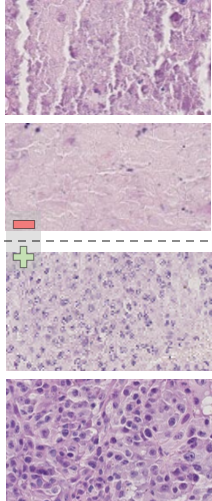
\includegraphics[width=\textwidth]{mtask/illus_necrose.png}
        \caption{Necrosis}
    \end{subfigure}
    \begin{subfigure}[t]{0.115\textwidth}
        \centering
        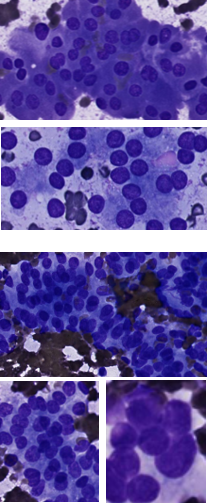
\includegraphics[width=\textwidth]{mtask/illus_patterns.png}
        \caption{ProliferativePattern}
    \end{subfigure}
    \begin{subfigure}[t]{0.115\textwidth}
        \centering
        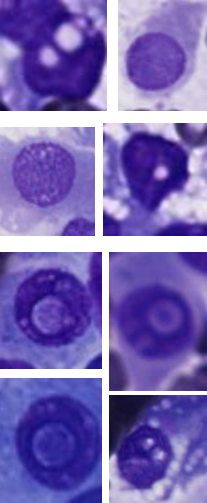
\includegraphics[width=\textwidth]{mtask/illus_cells.png}
        \caption{CellInclusion}
    \end{subfigure}
    \begin{subfigure}[t]{0.115\textwidth}
        \centering
        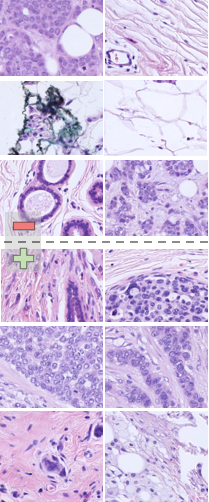
\includegraphics[width=\textwidth]{mtask/illus_breast.png}
        \caption{Breast}
    \end{subfigure}
    \begin{subfigure}[t]{0.115\textwidth}
        \centering
        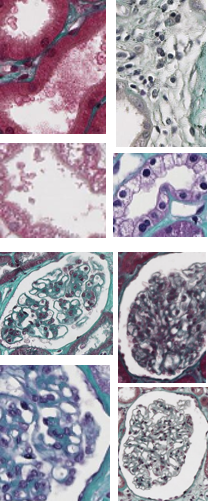
\includegraphics[width=\textwidth]{mtask/illus_glomeruli.png}
        \caption{Glomeruli}
    \end{subfigure}
    \begin{subfigure}[t]{0.115\textwidth}
        \centering
        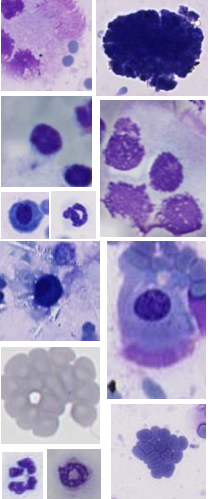
\includegraphics[width=\textwidth]{mtask/illus_lbtd_lba.png}
        \caption{MouseLba}
    \end{subfigure}
    \begin{subfigure}[t]{0.115\textwidth}
        \centering
        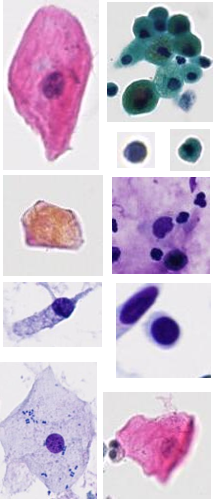
\includegraphics[width=\textwidth]{mtask/illus_anapath.png}
        \caption{HumanLba}
    \end{subfigure}
    \begin{subfigure}[t]{0.115\textwidth}
        \centering
        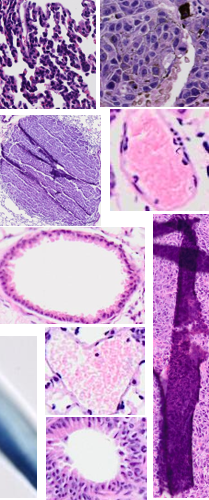
\includegraphics[width=\textwidth]{mtask/illus_tissus.png}
        \caption{Lung}
    \end{subfigure} \\
    \begin{subfigure}[t]{0.115\textwidth}
        \centering
        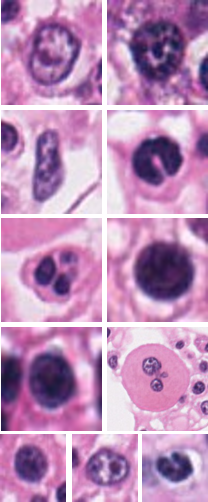
\includegraphics[width=\textwidth]{mtask/illus_bonemarrow.png}
        \caption{BoneMarrow}
    \end{subfigure}    
    \begin{subfigure}[t]{0.115\textwidth}
        \centering
        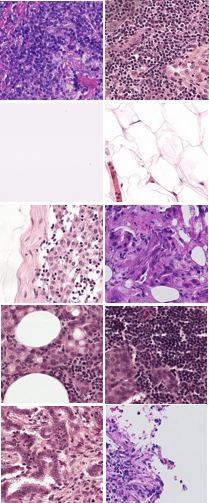
\includegraphics[width=\textwidth]{mtask/illus_camelyon16.png}
        \caption{Camelyon 16}
    \end{subfigure}
    \begin{subfigure}[t]{0.115\textwidth}
        \centering
        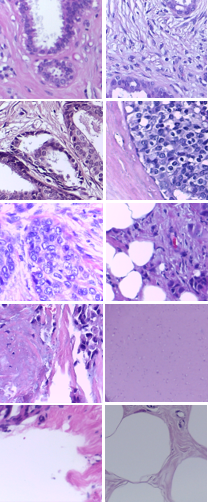
\includegraphics[width=\textwidth]{mtask/illus_bach18.png}
        \caption{BACH18 Micro}
    \end{subfigure}
    \begin{subfigure}[t]{0.115\textwidth}
        \centering
        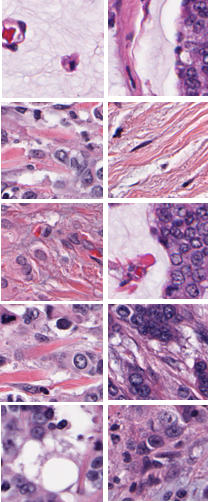
\includegraphics[width=\textwidth]{mtask/illus_janowczyk1.png}
        \caption{Janowczyk1}
    \end{subfigure}
    \begin{subfigure}[t]{0.115\textwidth}
        \centering
        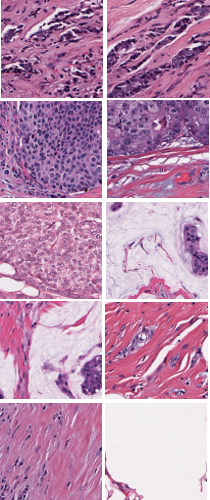
\includegraphics[width=\textwidth]{mtask/illus_janowczyk2.png}
        \caption{Janowczyk2}
    \end{subfigure}
    \begin{subfigure}[t]{0.115\textwidth}
        \centering
        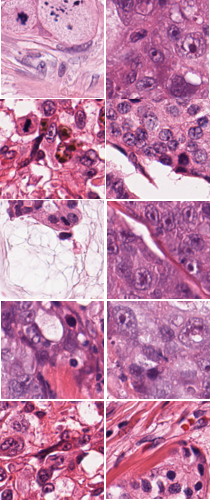
\includegraphics[width=\textwidth]{mtask/illus_janowczyk5.png}
        \caption{Janowczyk5}
    \end{subfigure}
    \begin{subfigure}[t]{0.115\textwidth}
        \centering
        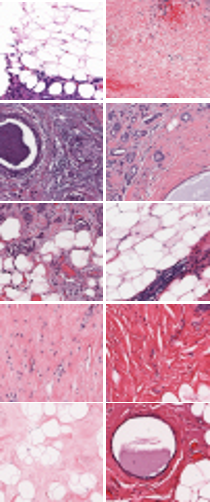
\includegraphics[width=\textwidth]{mtask/illus_janowczyk6.png}
        \caption{Janowczyk6}
    \end{subfigure}
    \begin{subfigure}[t]{0.115\textwidth}
        \centering
        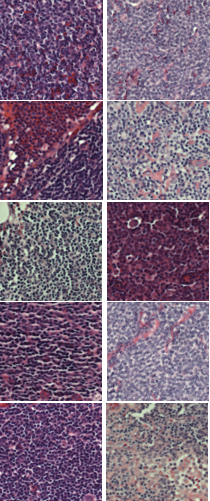
\includegraphics[width=\textwidth]{mtask/illus_janowczyk7.png}
        \caption{Janowczyk7}
    \end{subfigure} \\
    \begin{subfigure}[t]{0.115\textwidth}
        \centering
        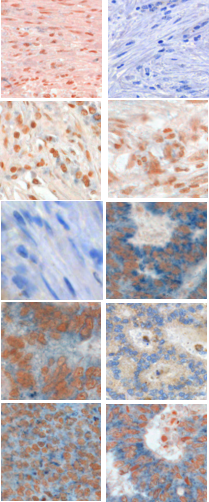
\includegraphics[width=\textwidth]{mtask/illus_lbpstroma.png}
        \caption{Stroma LBP}
    \end{subfigure}
    \begin{subfigure}[t]{0.115\textwidth}
        \centering
        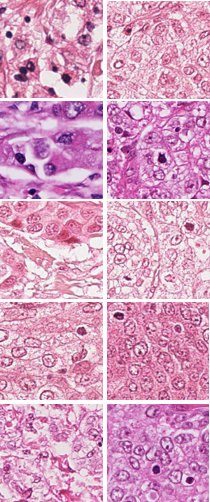
\includegraphics[width=\textwidth]{mtask/illus_mitos14.png}
        \caption{MITOS-ATYPIA}
    \end{subfigure}
    \begin{subfigure}[t]{0.115\textwidth}
        \centering
        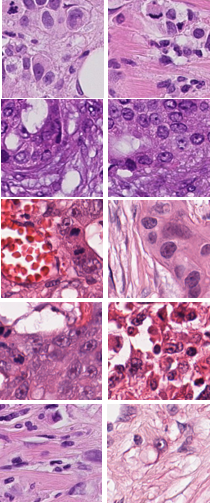
\includegraphics[width=\textwidth]{mtask/illus_tupac.png}
        \caption{TUPAC2016 Mitosis}
    \end{subfigure}
    \begin{subfigure}[t]{0.115\textwidth}
        \centering
        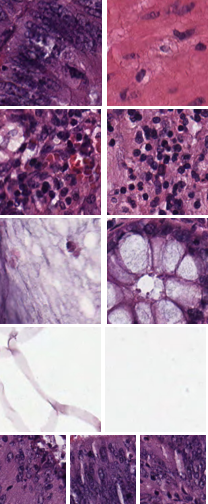
\includegraphics[width=\textwidth]{mtask/illus_umcm.png}
        \caption{UMCM Colorectal}
    \end{subfigure}
    \begin{subfigure}[t]{0.115\textwidth}
        \centering
        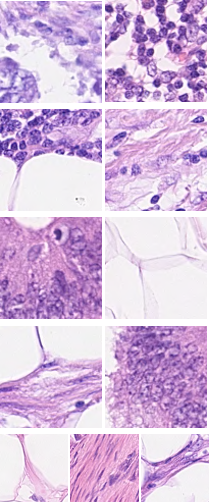
\includegraphics[width=\textwidth]{mtask/illus_warwick.png}
        \caption{Warwick CRC}
    \end{subfigure}
    \caption{Overview of our final classification tasks (the display size does not reflect actual image size). In this figure, we provide only one set of selected samples for Breast1 and Breast2 as their corresponding tasks are similar and they originate both from the same set of WSIs.}
    \label{fig:mtask:dataset_samples}
\end{figure*}

For the collected datasets to be used in a multi-task classification setting, some dataset-specific pre-processing procedures had to be executed on most of them. Applying those procedures, we have constructed a pool of 22 classification tasks which contains both binary and multiclass classification problems. The different pre-processing are detailed in Supplementary Section \ref{app:mtask:sec:datasets}. Whereas we have tried to avoid intra-dataset class imbalance, there is major inter-dataset imbalance regarding the number of images: the smallest dataset contains 882 images whereas the largest one contains almost 300k. However, we believe it is not an issue and can be made of minor significance by adopting an ad-hoc multi-task training protocol (see Section \ref{ssec:mtask:multitask-training}). Selected samples of the final tasks are provided in Figure \ref{fig:mtask:dataset_samples}. 

\section{Methods}
\label{sec:mtask:methods}

\begin{figure}
    \centering
    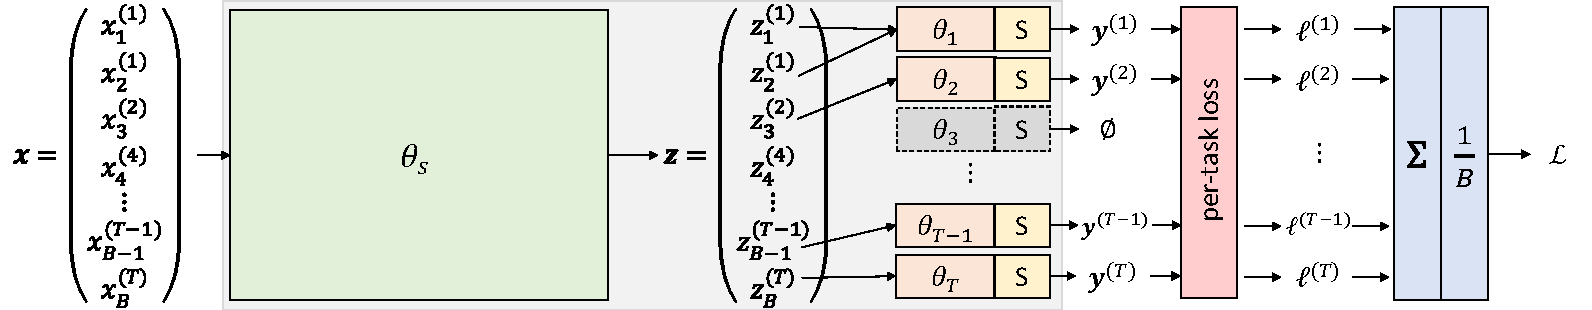
\includegraphics[width=\textwidth]{mtask/multitask-training.pdf}
    \caption{Multi-task architecture. $\mathcal{L}$ is the multi-task loss (see Section \ref{ssec:mtask:multitask-training}) and $S$ is a softmax layer. $x_j^{(i)}$ and $z_j^{(i)}$ designate respectively the $j^{\text{th}}$ sample of the batch $\mathbf{x}$ and its corresponding features produced by $\theta_s$. This sample belongs to task $t_i$. Features produced for samples of a given task $t_i$ are routed to this task head $\theta_i$. In this example, there is no sample for task 3 in the batch $\mathbf{x}$. Therefore, the corresponding head $\theta_3$ is inactive (\ie produces no output, no parameters update, no gradient computed) for this iteration.}
    \label{fig:mtask:multitask-training}
\end{figure}

In the following section, we present the training and evaluation protocols and the experiments we have carried out. Those experiments have two main objectives. The first is to evaluate how performance of multi-task and ImageNet pre-trained networks compare when transferred to a target task. The second is to better understand how various training hyperparameters and choices impact the transfer of a multi-task pre-trained network. The multi-task architecture and training are described in \ref{ssec:mtask:multitask-architecture} and \ref{ssec:mtask:multitask-training}. We present the different transfer techniques we have used in Section \ref{ssec:mtask:transfer_techniques}. We have developed a model evaluation and selection protocol which is described in Sections \ref{ssec:mtask:exp:transfer_eval} and \ref{ssec:mtask:exp:model_eval} whereas the various parameters we have chosen and/or evaluated as well as the experiments we have carried out are presented in Section \ref{ssec:mtask:exp:parameters}. 

Regarding notations, we consider a multi-task setting with a pool $\mathcal{P}$ of $T$ classification tasks. Each task $\mathcal{D}_i$ has $n_{i}$ training samples and its classification problem features $C_{i}$ classes. $\mathcal{B}$ represents the set containing all samples from a batch and the batch size is denoted by $B = \left|\mathcal{B}\right|$. $\mathcal{B}_{i} \subseteq \mathcal{B}$ is a set that contains all the samples from task $\mathcal{D}_i$ in batch $\mathcal{B}$. 

\subsection{Multi-task architecture}
\label{ssec:mtask:multitask-architecture}

The structure of our multi-task neural network is similar to those of \cite{shang2019and} and \cite{strezoski2019many} and is guided by the objective of pre-training a network for transfer. Therefore, we have adopted the architecture presented in Figure \ref{fig:mtask:multitask-training}. The to-be transferred network is shared for all tasks and denoted by $\theta_s$. We attach a head $\theta_i$ to $\theta_s$ for each task $\mathcal{D}_i$ in the pool $\mathcal{P}$. The head $\theta_i$ is simply a fully connected layer of dimensions $f_s\times C_{i}$ where $f_s$ is the number of features produced by $\theta_s$. Using such a simple layer has the benefit of making the learning capacity of the heads much lower compared to the shared network (in our experiments $|\theta_s| \gg |\theta_i|, \forall i$), hence forcing $\theta_s$ to learn relevant features for all tasks. In each head, a softmax is attached after the fully connected layer for producing per-task predictions. When forwarding samples in the multi-task network, samples of a given task $\mathcal{D}_i$ are only routed through the head $\theta_i$, which outputs predictions for those samples. 

\subsection{Multi-task training}
\label{ssec:mtask:multitask-training}

Classical training choices have to be adapted for the multi-task setting. Regarding batch sampling, we have decided to interleave tasks at the sample level, meaning that a single batch can contain samples from different tasks. Indeed, we believe that if batches containing samples from only a single task were alternated, the network would not see a particular task for $T-1$ iterations, with $T$ the number of tasks, which could make the training harder when $T$ is large.

Given the imbalance in terms of number of images per task, a batch sampling procedure had to be carefully established. Indeed, a simple random sampling across all images would prevent the tasks with fewer images from being seen during training. To overcome this issue, we selected each image in a batch by first randomly sampling a task and then sampling an image from this task, thus giving equal weights to all tasks.

Regarding the training loss, we averaged the categorical cross-entropy over all batch samples taking into account their respective tasks. More precisely, the multi-task loss $\mathcal{L}$ is computed from a batch as:
\begin{equation}\label{eqn:loss}
\mathcal{L} = \frac{1}{B} \sum_{i=1}^T \ell^{(i)}, \ell^{(i)} = - \sum_{j=1}^{\left|\mathcal{B}_{i}\right|} \sum_{k=1}^{C_{i}} y^{(i)}_{j,k} \log \hat{y}^{(i)}_{j,k}
\end{equation}
where $\ell^{(i)}$ is the loss for the batch samples from task $\mathcal{D}_i$.

When developing a multi-task algorithm, a crucial question is what should be shared between tasks. By reducing the capacity of the heads of our architecture, we wanted to enforce the training algorithm to find generic features in $\theta_s$ that work well for all tasks. It might be interesting however to provide a way to slightly relax this implicit constraint, with a hyperparameter. To this end, during training, whereas we train the network with a learning rate $\gamma$, we choose to train the heads with a potentially different learning rate given by $\gamma_h = \gamma \times \tau_\gamma$ where $\tau_\gamma \in \mathbb{R}_{\geq0}$ is a multiplicative factor applied to the global learning rate. This new hyperparameter provides a way of tuning the specificity/genericity of the learned shared features.  Indeed, $\tau_\gamma > 1$ makes the heads learning rate larger and gives therefore more flexibility for the heads to adapt, hence relieving the shared network from learning task-specific features. Taking $\tau_\gamma = 1$ results in using the same learning rate for the whole network.

As previously mentioned, each head $\theta_i$ is randomly initialized, whereas we initialize $\theta_s$ with ImageNet pre-trained weights as it has been shown that doing so accelerates convergence in a single-task setting \cite{mormont2018comparison}. However, it means that trained features of $\theta_s$ are followed directly by the random layers of the heads. This is known to hurt performance in a single-task transfer setting as reported in \citeauthor{yosinski2014transferable} \cite{yosinski2014transferable} and is aggravated in a multi-task setting. Indeed, during the first training iterations, the heads gradients will be relatively large and will work to turn each head weights from random to relevant with respect to its task. However, the resulting back-propagated gradients in the last layer of $\theta_s$ will be an average of the potentially contradictory signals coming from all the heads. In order to attenuate or eliminate this problem, a simple idea consists in making each head weights relevant to its task before training the whole network by running a warm up phase during which $\theta_s$ is frozen (\ie no weights update, no batch normalization update) and only the heads $\theta_i$ are trained with a learning rate $\gamma_w$. 

While preparing our experiments, we have noticed two issues: one with batch normalization \cite{ioffe2015batch} and one with the heads gradients. The former is a consequence of the \acrlong{tl} settings whereas the second is a consequence of the task-based routing of samples in the heads. Both are discussed below.

\subsubsection{Issue with batch normalization} 
\label{sssec:mtask:batchnormissue}

It has been shown that a network equipped with batch normalization \cite{ioffe2015batch} can exhibit issues when it is used across different domains \cite{li2018adaptive, chang2019domain}. A similar issue occurs when transferring such network to one or several target tasks of which the input distributions differs greatly from the source task. Indeed, the first iteration will propagate through the network samples from an unseen and likely different distribution which will trigger a massive change of batch normalization module statistics ($\mu_\mathcal{B}$ and $\sigma_\mathcal{B}$). However, the batch normalization trainable parameters ($\beta$ and $\gamma$) will themselves be updated much more slowly (especially when the training learning rate is small) preventing them to adapt properly to the shift in distribution and statistics. 

In the context of this work, early experiments have shown that it had an undesirable negative effect on training basically destroying the purpose of transfer, as the training curves exhibited a similar behavior to training from scratch. This problem was aggravated in multi-task learning when several tasks, with different input distributions, were used. We have applied a simple procedure to attenuate this effect. Our idea consists in updating parameters $\beta$ and $\gamma$ of each batch normalization module before starting training such that the output of the module is preserved when the shift in distribution occurs. Given a source task $\mathcal{D}_s$ and a target task $\mathcal{D}_t$, few batches of the target task are forwarded into the network to estimate the new statistics $\mu_{\mathcal{B}_t}$ and $\sigma_{\mathcal{B}_t}$ of each batch normalization module input. Based on the obtained statistics, the new parameters $\beta_s$ and $\gamma_s$ for a module are given by (see below for the derivation of these formulas):
\begin{eqnarray}
\gamma_t &=& \gamma_s \dfrac{\sigma^{(\epsilon)}_{\mathcal{B}_t}}{\sigma^{(\epsilon)}_{\mathcal{B}_s}}\label{app:mtask:eqn:bn_update_gamma}\\
\beta_t &=& \beta_s + \gamma_s  \dfrac{(\mu_{\mathcal{B}_t}-\mu_{\mathcal{B}_s})}{\sigma^{(\epsilon)}_{\mathcal{B}_s}}\label{app:mtask:eqn:bn_update_beta}
\end{eqnarray}
where $\mu_{\mathcal{B}_s}$, $\sigma^{(\epsilon)}_{\mathcal{B}_s}$, $\beta_s$ and $\gamma_s$ are the original source task's statistics and parameters. The expression $\sigma^{(\epsilon)}_{\mathcal{B}_x}$ denotes an altered version of standard deviation presented in the original paper which is given by $\sqrt{\sigma_{\mathcal{B}_x}^2 + \epsilon}$ with a $\epsilon$ constant added for numerical stability. In our multi-task setting, we have used batches containing samples from all tasks during the new statistics estimation in order to mimic the actual inputs distributions at training time.

\paragraph{Deriving the formulas} A batch normalization module being a composition of linear functions, it is therefore linear and can be re-expressed as:
\begin{equation} \label{app:mtask:eqn:batch_norm_is_linear}
y_k = BN_k(x) = m_k x + p_k
\end{equation}
where $y_k$ and $x$ respectively denote the output of the batch normalization module for task $k$ (\ie using task $k$ statistics and parameters) and the input of the batch normalization module. Using the definition of the module, Equation \ref{app:mtask:eqn:batch_norm_is_linear} can be rewritten as:
\begin{equation} \label{app:mtask:eqn:batch_norm_is_linear_rewritten}
y_k = \underbrace{\dfrac{\gamma_k}{\sigma^{(\epsilon)}_{\mathcal{B}_k}}}_{m_k} x + \underbrace{\beta_k - \gamma_k\ \dfrac{\mu_{\mathcal{B}_k}}{\sigma^{(\epsilon)}_{\mathcal{B}_k}}}_{p_k}.
\end{equation}
The formula in Equations \ref{app:mtask:eqn:bn_update_gamma} and \ref{app:mtask:eqn:bn_update_beta} are obtained by ensuring $y_t = y_s$ for any $x$, or similarly solving the following system:
\begin{align}
\begin{cases}
m_s = m_t\\
p_s = p_t\\
\end{cases}
\end{align}

\subsubsection{Issue with heads gradients}
\label{sssec:mtask:gradientissue}

Because samples are routed through their respective task head in our architecture, all parts of the network do not see the same number of samples from a batch which causes the gradients to be underestimated in the network heads. This can be shown by developing the derivative of our loss with respect to one of the logits of a head. Let $r^{(i)}_{k}$ be the class $k$ logit of task $t_i$. The derivatives of the loss ${\cal L}$ (Equation 1, in the original publication) with respect to $r^{(i)}_k$ is given by:
\begin{equation} 
    \label{app:mtask:eqn:rescale_grad}
    \frac{\partial \mathcal{L}}{\partial r^{(i)}_{k}} = - \frac{1}{B} \sum_{j=1}^{\left|\mathcal{B}_{t_i}\right|} \frac{\partial \ell^{(i)}_j}{\partial r^{(i)}_{k}},
\end{equation}
where $\ell^{(i)}_j$ is the loss term for the $j$th sample of task $t_i$ in the batch sample. Equation \ref{app:mtask:eqn:rescale_grad} shows that the gradients are divided by the batch size although they are estimated using $\left|\mathcal{B}_{t_i}\right|$ samples (\ie the number of samples from task $t_i$ in the batch). This applies also to the gradients used for updating the parameters $\theta_i$ of the head. Given a task $t_i$, this magnitude reduction has the same effect as dividing the learning rate for head $\theta_i$ by a variable factor that depends on the number of samples of task $t_i$ that are present in the batch. If tasks are sampled uniformly to create a batch, one can expect this factor to be equal to the number of tasks $T$ on average. In order to avoid this phenomenon, we applied a simple trick that consists in re-scaling the gradients of each head $\theta_i$ by multiplying them by $\phi_{t_i}$:
\begin{equation}
\phi_{t_i} = \frac{B}{\left|\mathcal{B}_{t_i}\right|}.
\end{equation}


%% Equation \ref{app:mtask:eqn:rescale_grad} can be derived by developing the derivative of the loss by the logits of one head:

%% \begin{align}
%%     \frac{\partial \mathcal{T}}{\partial r^{(i)}_{k}} &= \frac{\partial}{\partial r^{(i)}_{k}} \left[- \frac{1}{B} \sum_{m=1}^T \sum_{j=1}^{\left|\mathcal{B}_{t_m}\right|} \ell^{(m)}_j \right] \\
%%     &= - \frac{1}{B} \sum_{j=1}^{\left|\mathcal{B}_{t_i}\right|} \frac{\partial \ell^{(i)}_j}{\partial r^{(i)}_{k}} \\
%% \end{align}

% \[
%   \frac{B}{\left|\mathcal{B}_{t_i}\right|} \frac{\partial \mathcal{T}}{\partial r^{(i)}_{k}} = -  \frac{1}{\left|\mathcal{B}_{t_i}\right|} \sum_{j=1}^{\left|\mathcal{B}_{t_i}\right|} \frac{\partial \ell^{(i)}_j}{\partial r^{(i)}_{k}} 
% \]

\subsection{Transferring a multi-task pre-trained network}
\label{ssec:mtask:transfer_techniques}

We study both deep \acrlong{tl} approaches, namely feature extraction and fine-tuning. In both cases, $\theta_s$ is pre-trained on some source task(s), either ImageNet or several tasks simultaneously in the \acrshort{mtl} setting. For feature extraction, we exclusively use the pre-trained network $\theta_s$ to extract features for all images of the target task. The extracted features can then be used to learn a third-party classifier, a common choice being a linear \acrshort{svm}. For fine-tuning, we further train the shared network $\theta_s$ on the target task by attaching to it a fully connected layer and a softmax. The resulting network is trained using for instance stochastic gradient descent

Both approaches have their own complementary advantages and drawbacks. As mentioned above, feature extraction uses a linear model which is very fast to train and makes it robust to overfitting when working with small target datasets. However, using fixed pre-trained features makes it possible that the features are not entirely suited for the target task (\eg ImageNet vs. \acrlong{dp}), yielding suboptimal performance. Fine-tuning does not suffer from this drawback as the whole network (or a part of it) is retrained on the target task. When using large capacity networks (\eg ResNet or DenseNet), it allows the network to capture and learn task-specific features. This is however an issue when the target dataset is small because the large capacity of the network can lead to overfitting.

\subsection{Evaluating transferability for hyperparameter tuning}
\label{ssec:mtask:exp:transfer_eval}\label{ssec:mtask:exp:model_selection}

Given a set of tasks available to pre-train a \acrshort{mtl} model for future transfer, either by feature extraction or fine-tuning, a question left is how to tune the hyperparameters to train this model. Since we want to optimize the transferability of the model, rather than for example its average performance on the training tasks, we have to design a specific evaluation protocol and a specific metric to assess this transferability for each hyperparameter combination.

For this purpose, we have developed a leave-one-task-out (LOTO) cross-validation scheme, inspired from leave-one-out cross-validation. It consists in removing a set $\mathcal{T} \subset \mathcal{P}$ of one or more tasks from the training pool $\mathcal{P}$, training a multi-task model on $\mathcal{P} \setminus \mathcal{T}$ and then evaluating how the learnt models transfer to the tasks of $\mathcal{T}$. This operation can then be repeated for different $\mathcal{T}$ to increase the stability of the analysis. In our case, we have picked $\mathcal{T}$ to contain only one task when possible. However, it is important that tasks that are closely related are left out together during LOTO cross-validation to avoid data leakage. In our case, there are two pairs of datasets that are subject to this exception. The first is CellInclusion and ProliferativePattern which are different classification tasks coming from the same WSIs. The second is Breast1 and Breast2 which are the same classification tasks generated with different rules from the same expert annotations. Therefore, applying LOTO exhaustively in our settings leads to 20 possible left out sets $\mathcal{T}$. 

The optimal hyperparameter combination might arguably depend on whether the \acrshort{mtl} model will be used for feature extraction or fine-tuning. We have however solely used feature extraction performance as a proxy to evaluate transferability, mainly because we wanted to release a single \acrshort{mtl} model for simplicity, but also to reduce the computational costs of our experiments. More precisely, given a left-out set $\mathcal{T}$ and one of its task $\mathcal{D} \in \mathcal{T}$, we have evaluated transferability of a multi-task pre-trained network trained on $\mathcal{P} \setminus \mathcal{T}$ by using the resulting $\theta_s$ as a feature extractor on $\mathcal{D}$. The training set of $\mathcal{D}$ was used to train the features classifier (\ie a linear \acrshort{svm}, see Section \ref{ssec:mtask:exp:parameters} for details) and the validation set was used to evaluate it. Transfer performance was evaluated by the \acrfirst{acc} for multi-class classification tasks and the area under the receiver operating characteristic curve \rocauc for binary classification tasks. To cope with the randomness induced by heads initialization and mini-batch sampling, each training of a \acrshort{mtl} model was repeated with 5 different random seeds. Note that, at this stage, the test set of $\mathcal{D}$ was kept aside for future comparison of a selected multi-task pre-trained network and comparison to ImageNet transfer (see Section \ref{ssec:mtask:exp:model_eval}).

All the scores resulting from the same hyperparameters combination but different random seeds can be averaged and the resulting average performance can be used to assess transfer performance on a given task $\mathcal{D}$. We need however to aggregate these scores over all (left-out) tasks to assess the overall transferability of a given hyperparameter combination. Averaging ACC and ROC AUC scores over tasks is in general not a good idea as these values depends on the task difficulty and are not directly comparable across tasks. We propose instead to aggregate rankings. More precisely, for each task, the combination of hyperparameters leading to the best model on average was assigned rank $1$ and the worst was assigned the maximum rank. Applying this procedure to all our sets $\mathcal{T}$ produces a rank matrix where $r_{ij}$ is the rank of the $i^{\text{th}}$ combination of hyperparameters evaluated on the left-out task $j$. The best hyperparameter combination is then defined as the one that minimizes the average rank over all left-out tasks:
\begin{equation} \label{eqn:average_ranks}
\overline{r}_i = \dfrac{1}{T_{\text{out}}} \sum^{T_{\text{out}}}_{j = 1} r_{ij}
\end{equation}
where $T_{\text{out}}$ is the number of left-out tasks.

\subsection{Final performance evaluation}
\label{ssec:mtask:exp:model_eval}

Our main objective is to compare transfer from multi-task and ImageNet pre-trained networks. In principle, two nested LOTO cross-validation loops should be adopted to carry out such comparison:  for each left-out task in the external LOTO CV loop, an additional internal LOTO CV loop should be run to find the optimal hyperparameter combination for training the \acrshort{mtl} model to be transferred to the (external) left-out task. Using two nested loops would be however too expensive computationally\footnote{The simplified scheme we present hereafter has already yielded approximately 20k GPU hours of computation. This computation time would have been multiplied by 10 using two nested LOTO CV loops, which was impossible for us to carry out given our available computing resources.}. We have instead adopted the following simplified scheme. A single LOTO cross-validation is run as described in the previous section. Given a left-out task $\mathcal{D}_k$, we select the hyperparameter combination that minimizes the average rank but now excluding task $\mathcal{D}_k$ from the average computation (\ie excluding $r_{ik}$ from the calculation of $\overline{r}_i$ in Equation \ref{eqn:average_ranks}). All the models trained using this hyperparameters combination (\ie one per seed) are transferred to the target task $\mathcal{D}_k$ using both transfer protocols (\ie feature extraction or fine-tuning). The test set of $\mathcal{D}_k$ is used solely to evaluate the resulting transfer performance whereas the training and validation sets can be used by the transfer protocol, feature extraction or fine-tuning, for training and hyperparameter tuning (see Section \ref{ssec:mtask:exp:parameters}).

Unlike with a true double LOTO CV loop, the training and validation sets of the left-out task $\mathcal{D}_k$ are used, in our simplified scheme, to train some of the \acrshort{mtl} models that are transferred to the other tasks for computing the rankings of the hyperparameters combinations for these tasks. However, this is not expected to introduce any bias since the data from task $\mathcal{D}_k$ is neither used to decide on the optimal hyperparameter setting of the \acrshort{mtl} model transferred to $\mathcal{D}_k$ itself (since $r_{ik}$ is excluded from the computation of $\overline{r}_i$), nor to train this \acrshort{mtl} model.

\subsection{Hyperparameters settings and experiments}
\label{ssec:mtask:exp:parameters} 

\begin{table}
    \centering
    \begin{tabular}{|rc|l|c|}
        \hline
        \multicolumn{2}{|c|}{Parameters} & Values & Count \\
        \hline
        Learning rate (LR) & $\gamma$ & $\{10^{-3}, 10^{-4}, 10^{-5}, 10^{-6}\}$ & 4 \\
        LR multiplier & $\tau_\gamma$ & $\{1, 5, 10\}$ & 3 \\
        Shared network & $\theta_s$ & $\{\text{ResNet50}, \text{DenseNet121}\}$ & 2 \\
        Warm up & $w$ & $\{true, false\}$ & 2 \\
        \hline
        \multicolumn{3}{|c|}{Number of combinations $\left|\mathcal{H}\right|$} & 48 \\
        \hline
        \multicolumn{3}{|c|}{with random seeds} & 240 \\
        \hline
    \end{tabular}
    \caption{The multi-task training parameters evaluated using the cross-validation procedure. Using the LOTO scheme, 240 trained models should be transferred to each left out dataset. $\mathcal{H}$ is the set of all hyperparameters combinations.}
    \label{tab:mtask:results:parameters}
\end{table}

The hyperparameters we have studied and their evaluated values are listed in Table \ref{tab:mtask:results:parameters}. Parameters values and training choices were established based on early experiments which evaluated multi-task training stability and convergence. Regarding the selected range of learning rates, values higher than $10^{-3}$ resulted in very unstable or diverging trainings whereas values lower than $10^{-6}$ prevented convergence. As shared network $\theta_s$, we have used two popular architectures ResNet50 \cite{he2016deep} and DenseNet121 \cite{huang2017densely}. We have removed the fully connected layer of those networks and replaced it by a global average pooling. Moreover, we have loaded the networks with ImageNet pre-trained weights from PyTorch \cite{paszke2019pytorch}.

The multi-task network was trained for 50k iterations using batches of size 64 and SGD as optimizer using momentum set to its default value (\ie $0.9$), learning rate $\gamma$ and heads learning rate multiplier $\tau_\gamma$. Either the whole network was trained directly, or the heads were first warmed up for 5k iterations with learning rate $\gamma_w = 10^{-3}$ before the whole network was trained for 45k iterations.

Classical data augmentation and normalization have been applied to the input images. We have used ImageNet statistics for normalizing the images as early experiments have shown no significant improvement by normalizing with per-task statistics. As data augmentation, we have applied simple random vertical and horizontal flips as well as extraction of a random square crop (if the image is not square already).

When feature extraction was applied either during the evaluation or selection, we have used linear \acrshort{svm} \cite{fan2008liblinear} as feature classifier. Whenever a \acrshort{svm} classifier was trained, we have tuned the $C$ regularization parameter among the following values $\left\{10^{-10}, 10^{-9},...,10^{-1},1\right\}$ by 5-fold cross-validation. The tasks were splitted into folds based on the most relevant information available for the task (patient, slide or image).

Regarding fine-tuning, we have trained the network for 100 epochs on the training set of the target task and have tuned the learning rate among $\{10^{-3}, 10^{-4}, 10^{-5}, 10^{-6}\}$ and have selected the best epoch on the validation set. When transferring from our multi-task pre-trained models, we have performed the selection of the best multi-task models as explained in Section \ref{ssec:mtask:exp:model_selection}. Then, for each model trained with the best hyperparameters (\ie one per seed), we have trained one model per fine-tuning hyperparameters combination. For ImageNet, the approach was slightly different as we had only one model to start from. In this case, we have used 5 different seeds for fine-tuning. 

At this point, it is important to note that LOTO cross validation is quite demanding in terms of computing resources as, for all $\mathcal{T}$, all the combinations of hyperparameters and random seeds have to be evaluated. As indicated in Table \ref{tab:mtask:results:parameters}, 240 models would have to be trained per set $\mathcal{T}$ of excluded tasks which, given 22 tasks, yields 4800 multi-task trainings. Due to limited availability of computing resources, we had to reduce this number and have done so by reducing the number of left out tasks used in our analysis. In particular, we have kept 10 tasks in 8 sets: $\{\text{CellInclusion}, \text{ProliferativePattern}\}$, $\{\text{Breast1}, \text{Breast2}\}$, $\{\text{MouseLba}\}$, $\{\text{HumanLba}\}$, $\{\text{Necrosis}\}$, $\{\text{Lung}\}$, $\{\text{Glomeruli}\}$ and $\{\text{BoneMarrow}\}$ (see Table \ref{tab:mtask:dataset_train_info}). All other tasks were always incorporated however to train each multi-task model.

For the sake of completeness, we have also compared the \acrlong{tl} approaches with training from scratch and joint training. The former consists in training a network initialized with random weights. The latter consists in training a network in multi-task using the whole pool of tasks (including the target tasks). 

For training from scratch, we have used the same settings as for the fine-tuning experiment except for the network weights initialization (using initialization strategy as defined in PyTorch): same evaluated learning rates, number of training epochs and same networks. Regarding joint training, we have used the same architecture and training algorithm as for our multi-task pre-training. For the evaluation tasks listed above, only their training set is used for the multi-task training, while their validation and test sets were respectively used for optimizing the hyperparameters and evaluating the selected model. The data for the other training tasks were kept the same as for multi-task pre-training.

\section{Results and discussion}
\label{sec:mtask:results}
\begin{figure}[t]
    \center
    \begin{subfigure}[t]{0.70\textwidth}
        \centering
        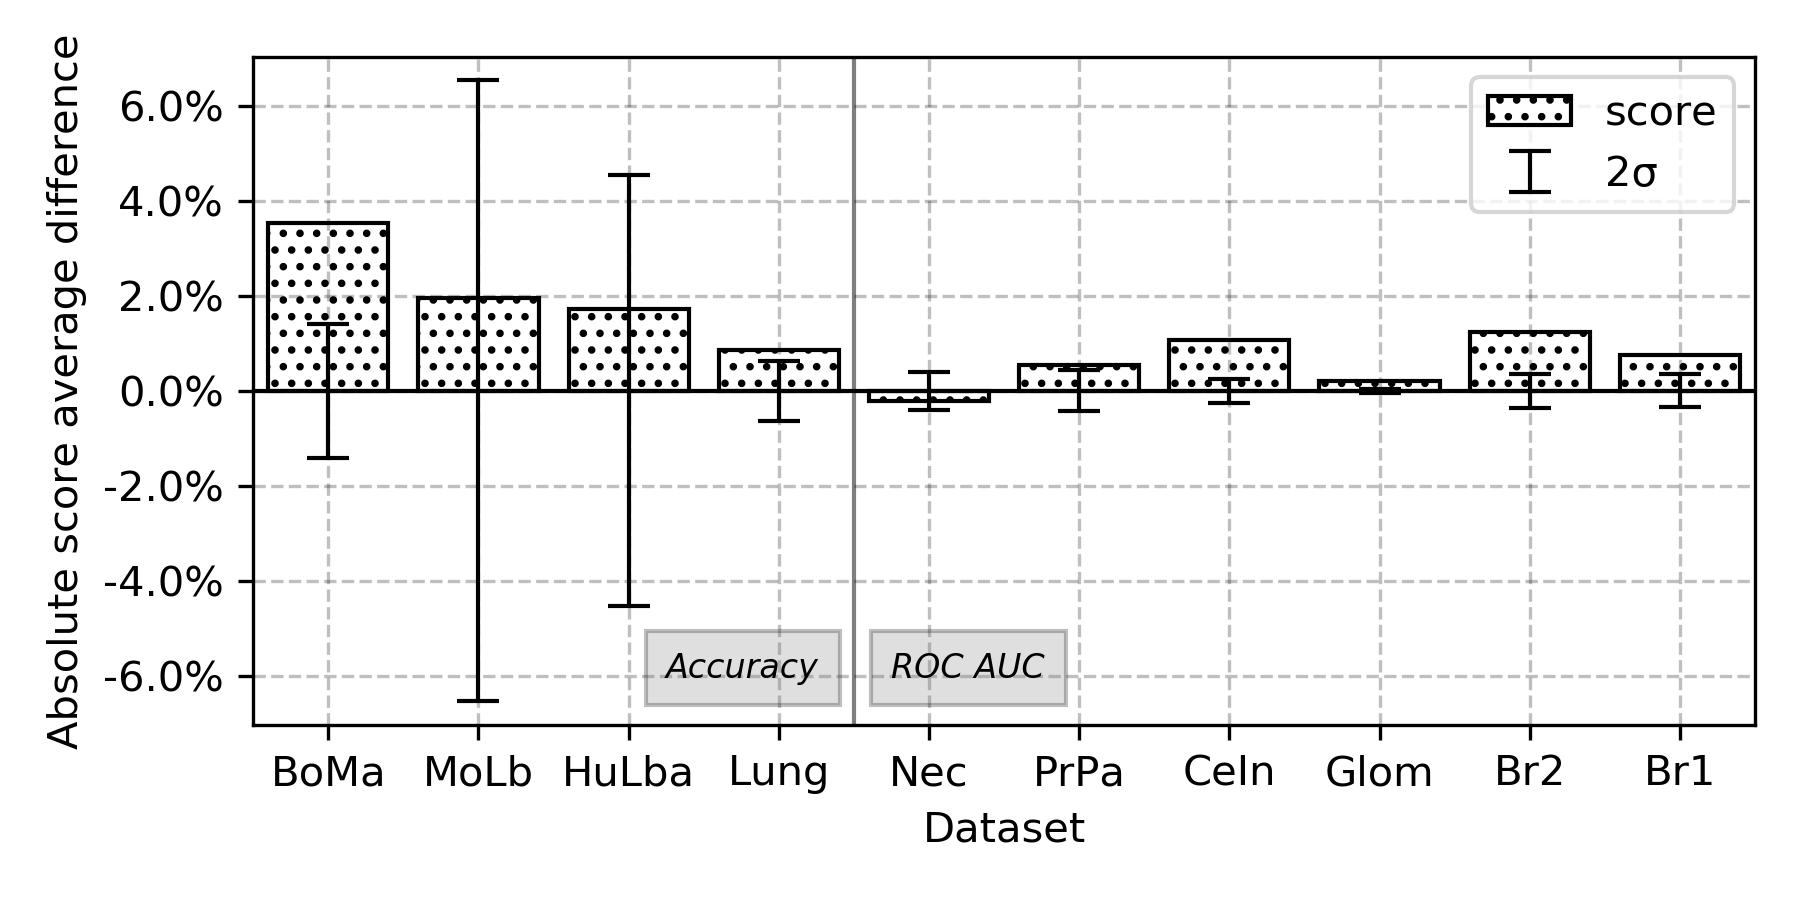
\includegraphics[width=\textwidth]{mtask/dense_fe.png}
        \caption{DenseNet121}
    \end{subfigure}    
    \begin{subfigure}[t]{0.70\textwidth}
        \centering
        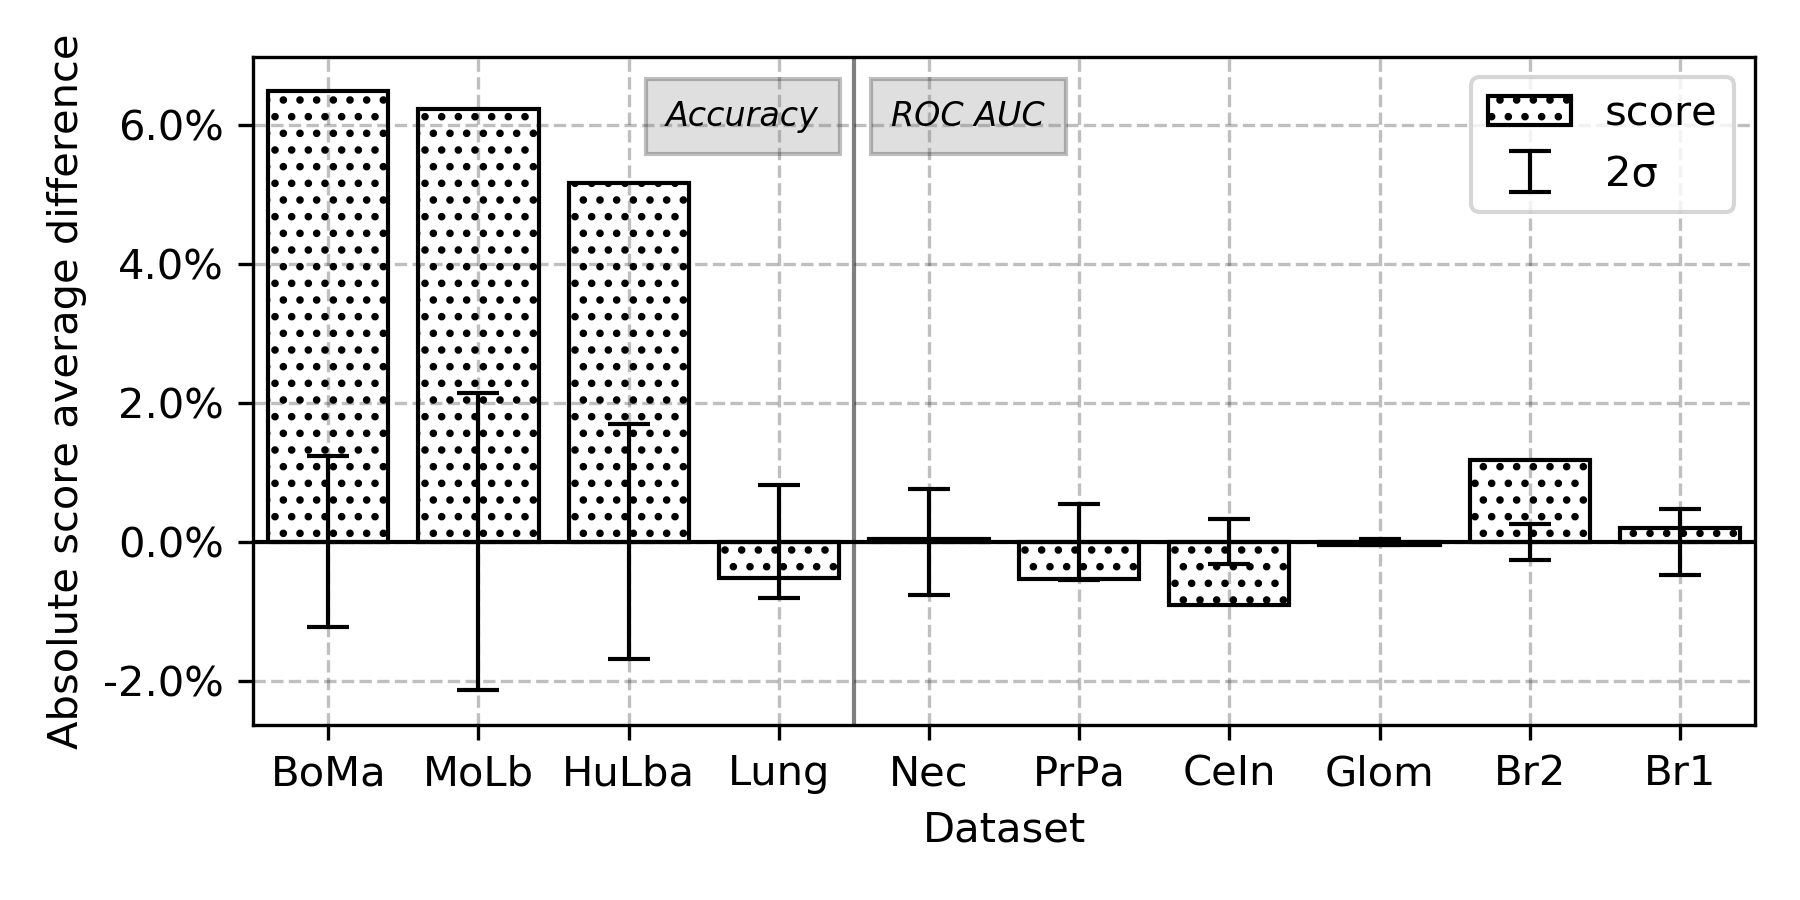
\includegraphics[width=\textwidth]{mtask/resnet_fe.png}
        \caption{ResNet50}
    \end{subfigure}    
    \caption{Absolute score difference between multi-task versus ImageNet pre-training using \textbf{feature extraction} as transfer protocol on our ten evaluation tasks. Positive difference indicates that multi-task pre-training yield superior performance. Tasks are sorted by evaluation metric and increasing dataset size. The variability of the multi-task transfer is measured using \textit{two} standard deviations given by the error bars.}  
    \label{fig:mtask:res_featext}
\end{figure}

\begin{figure}[t]
    \centering
    \begin{subfigure}[t]{0.70\textwidth}
        \centering
        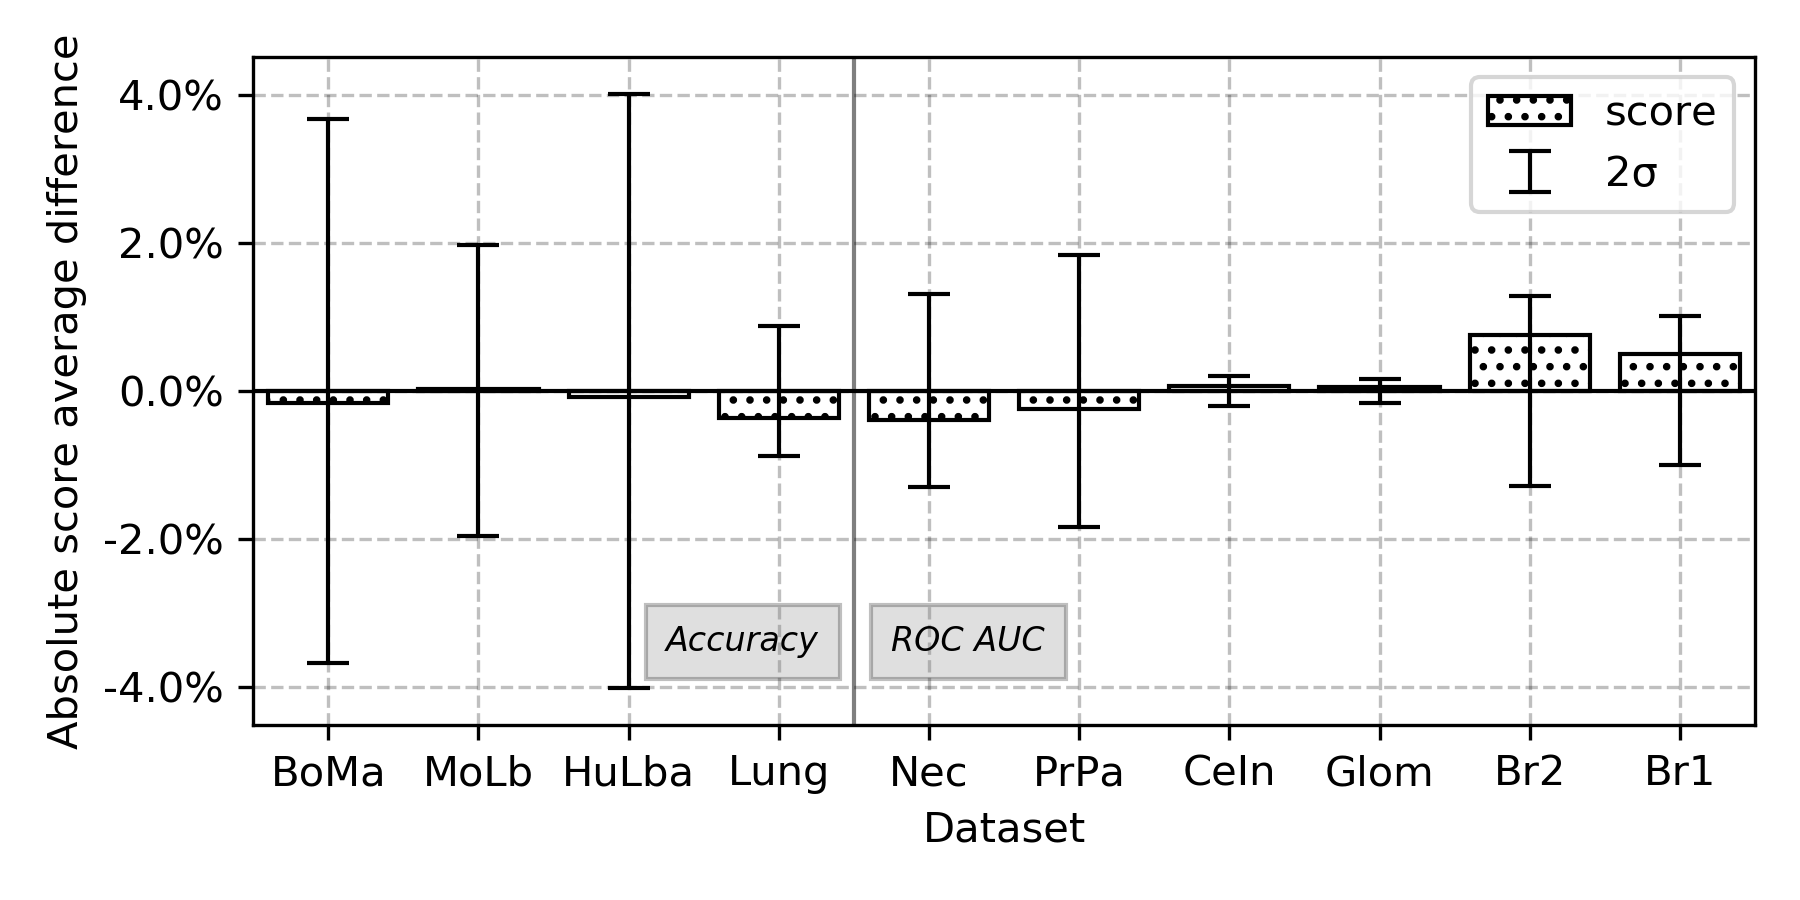
\includegraphics[width=\textwidth]{mtask/dense_ft.png}
        \caption{DenseNet121}
    \end{subfigure}    
    \begin{subfigure}[t]{0.70\textwidth}
        \centering
        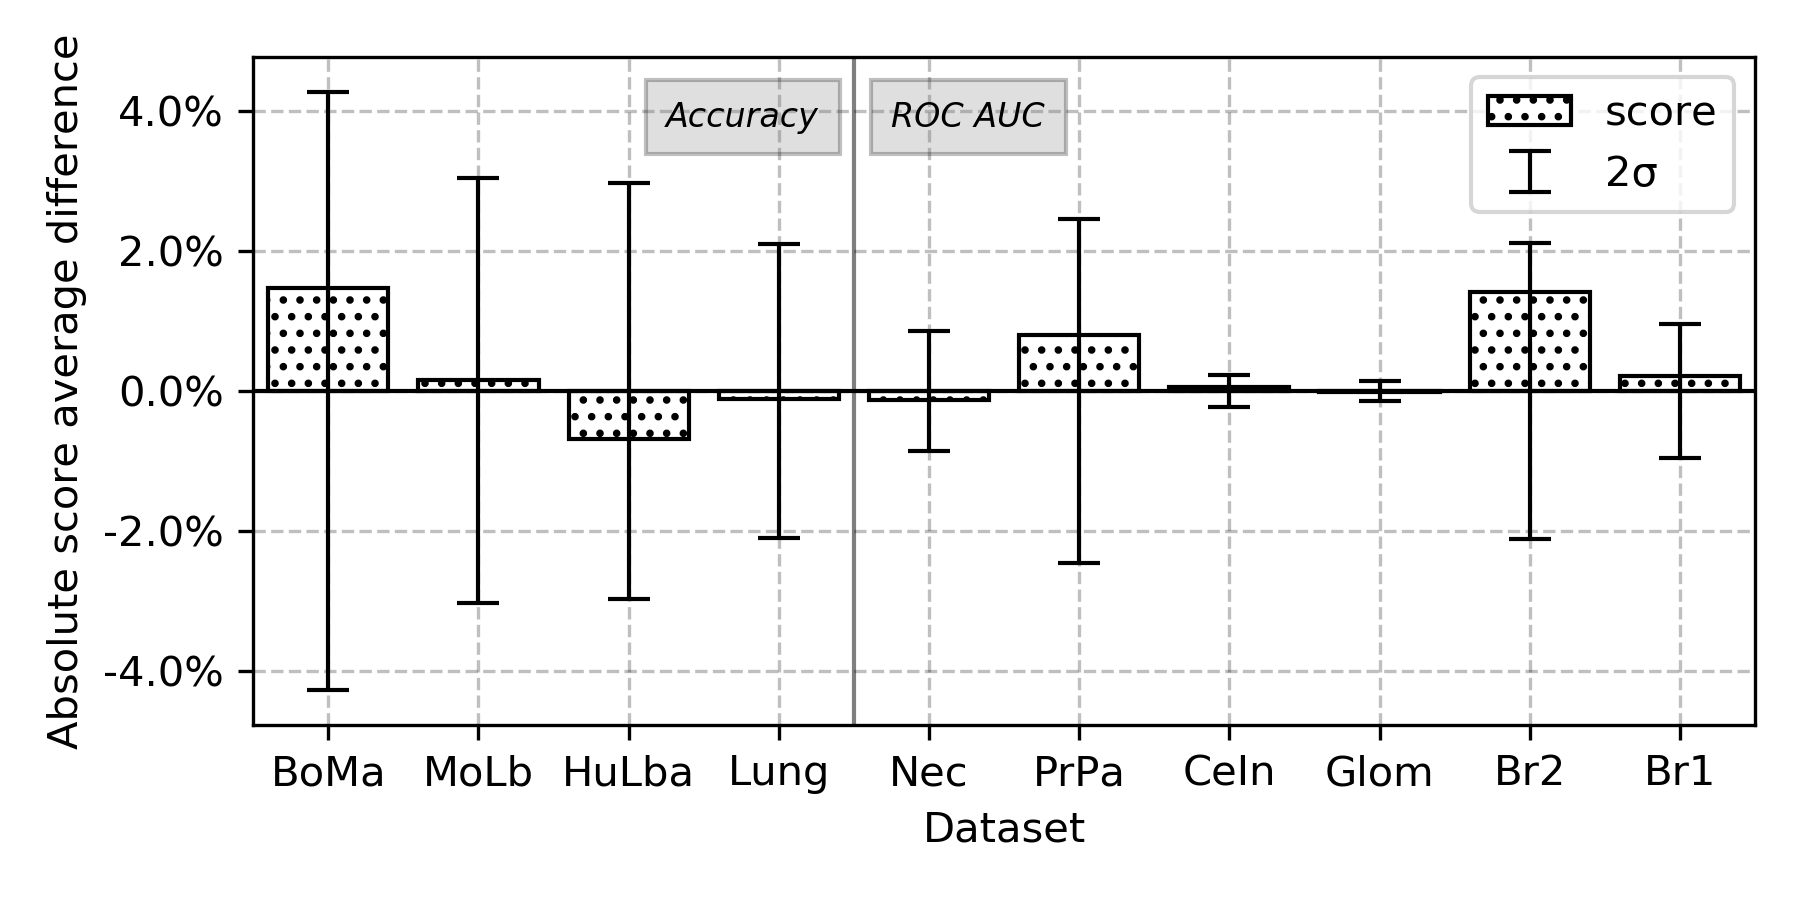
\includegraphics[width=\textwidth]{mtask/resnet_ft.png}\\
        \caption{ResNet50}
    \end{subfigure}    
    \caption{Absolute score difference between multi-task versus ImageNet pre-training using \textbf{fine-tuning} as transfer protocol on our ten evaluation tasks. See Figure \ref{fig:mtask:res_featext} for details. Error bars are computed using two times the largest standard deviation among the ones resulting from ImageNet and multi-task fine-tuning.}  
    \label{fig:mtask:res_finetune}
\end{figure}

\begin{figure}[t]
    \centering
    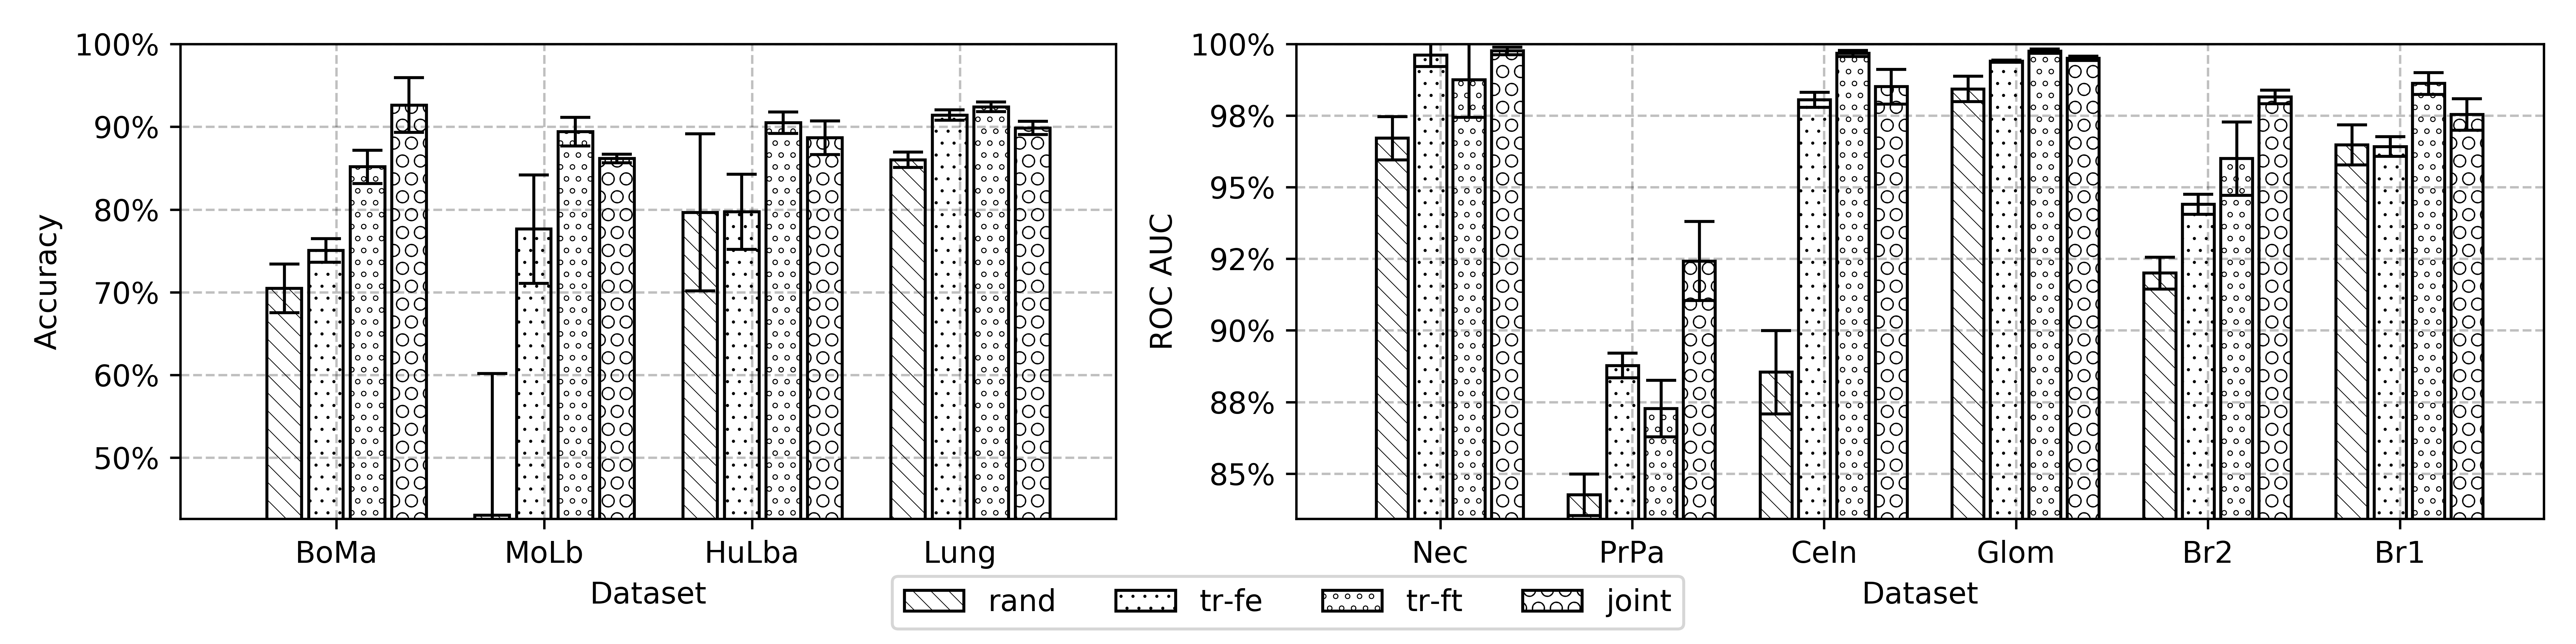
\includegraphics[width=\textwidth]{mtask/densenet_all.png}
    \caption{Performance comparison of different approaches using DenseNet121: training from scratch (\textit{rand}), feature extraction (\textit{tr-fe}) and fine-tuning (\textit{tr-ft}) using our multi-task pre-trained networks and joint training (\textit{joint}). Each bar is the average performance and its error bar gives twice the standard deviation of a given method over five runs. For exact scores, see Table \ref{tab:mtask:results_densenet}.}  
    \label{fig:mtask:res_all_densenet}
\end{figure}

\begin{table}[t]
    \centering
    \scriptsize
      \begin{tabular}{|c|c|c|c|c|c|c|c|c|}
      \hline
      & \textbf{Target} & \textbf{Train} &  \multirow{2}{*}{\textbf{Scratch}} & \multicolumn{2}{c|}{\textbf{Feature extraction}} & \multicolumn{2}{c|}{\textbf{Fine tuning}} & \multirow{2}{*}{\textbf{Joint training}} \\
      \cline{5-8}
      & \textbf{task} & \textbf{size} & & \textbf{ImageNet} & \textbf{Multi-task} & \textbf{ImageNet} & \textbf{Multi-task} & \\
      \hline
  \multirow{4}{*}{\rotatebox[origin=c]{90}{Accuracy}} & BoMa & 652 & $70.49 \pm 1.47$ & $71.52$ & $75.05 \pm 0.70$ & $85.32 \pm 1.84$ & $85.16 \pm 1.01$ & $92.62 \pm 1.66$ \\
  & MoLb & 2438 & $43.04 \pm 8.56$ & $75.68$ & $77.63 \pm 3.27$ & $89.39 \pm 0.98$ & $89.41 \pm 0.87$ & $86.17 \pm 0.26$ \\
  & HuLba & 4397 & $79.65 \pm 4.75$ & $78.01$ & $79.73 \pm 2.27$ & $90.56 \pm 2.01$ & $90.48 \pm 0.64$ & $88.67 \pm 1.01$ \\
  & Lung & 5443 & $86.01 \pm 0.47$ & $90.54$ & $91.40 \pm 0.32$ & $92.77 \pm 0.44$ & $92.41 \pm 0.29$ & $89.86 \pm 0.39$ \\
  \hdashline
  \multirow{6}{*}{\rotatebox[origin=c]{90}{ROC AUC}} & Nec & 791 & $96.71 \pm 0.38$ & $99.82$ & $99.61 \pm 0.20$ & $99.14 \pm 0.43$ & $98.75 \pm 0.65$ & $99.76 \pm 0.07$ \\
  & PrPa & 1346 & $84.26 \pm 0.36$ & $88.22$ & $88.77 \pm 0.21$ & $87.51 \pm 0.92$ & $87.27 \pm 0.49$ & $92.42 \pm 0.69$ \\
  & CeIn & 1816 & $88.54 \pm 0.73$ & $96.97$ & $98.05 \pm 0.13$ & $99.60 \pm 0.10$ & $99.67 \pm 0.05$ & $98.51 \pm 0.30$ \\
  & Glom & 14605 & $98.43 \pm 0.22$ & $99.20$ & $99.40 \pm 0.02$ & $99.70 \pm 0.08$ & $99.75 \pm 0.04$ & $99.50 \pm 0.04$ \\
  & Br2 & 14953 & $92.00 \pm 0.28$ & $93.17$ & $94.40 \pm 0.18$ & $95.24 \pm 0.59$ & $96.00 \pm 0.64$ & $98.15 \pm 0.12$ \\
  & Br1 & 18261 & $96.48 \pm 0.35$ & $95.66$ & $96.42 \pm 0.17$ & $98.12 \pm 0.50$ & $98.62 \pm 0.19$ & $97.54 \pm 0.27$ \\
      \hline
      \end{tabular}
      
      \caption{Performance of different evaluated approaches on DenseNet121. All reported scores are percentages. We compare training from scratch with feature extraction and fine-tuning from our multi-task pre-trained and the ImageNet models. We also provide results of the joint training experiment. Average performance and standard deviation are provided for all methods except for feature extraction from ImageNet as this procedure is deterministic.}
      \label{tab:mtask:results_densenet}
  \end{table}
  
  \begin{table}[t]
    \centering
    \scriptsize
      \begin{tabular}{|c|c|c|c|c|c|c|c|c|}
      \hline
      & \textbf{Target} & \textbf{Train} &  \multirow{2}{*}{\textbf{Scratch}} & \multicolumn{2}{c|}{\textbf{Feature extraction}} & \multicolumn{2}{c|}{\textbf{Fine tuning}} & \multirow{2}{*}{\textbf{Joint training}} \\
      \cline{5-8}
      & \textbf{task} & \textbf{size} & & \textbf{ImageNet} & \textbf{Multi-task} & \textbf{ImageNet} & \textbf{Multi-task} & \\
      \hline
  \multirow{4}{*}{\rotatebox[origin=c]{90}{Accuracy}} & BoMa & 652 & $65.88 \pm 1.16$ & $71.52$ & $78.00 \pm 0.61$ & $83.57 \pm 2.14$ & $85.04 \pm 0.37$ & $92.46 \pm 1.23$ \\
  & MoLb & 2438 & $48.47 \pm 4.19$ & $73.08$ & $79.31 \pm 1.07$ & $88.20 \pm 1.52$ & $88.36 \pm 1.27$ & $88.24 \pm 0.54$ \\
  & HuLba & 4397 & $71.85 \pm 8.33$ & $77.81$ & $82.97 \pm 0.84$ & $90.64 \pm 1.49$ & $89.95 \pm 0.61$ & $88.96 \pm 0.85$ \\
  & Lung & 5443 & $84.75 \pm 0.76$ & $91.67$ & $91.15 \pm 0.41$ & $92.73 \pm 0.33$ & $92.61 \pm 1.05$ & $90.89 \pm 0.35$ \\
  \hdashline
  \multirow{6}{*}{\rotatebox[origin=c]{90}{ROC AUC}} & Nec & 791 & $97.21 \pm 0.76$ & $99.17$ & $99.21 \pm 0.38$ & $99.21 \pm 0.34$ & $99.08 \pm 0.43$ & $99.81 \pm 0.10$ \\
  & PrPa & 1346 & $83.00 \pm 1.83$ & $90.00$ & $89.47 \pm 0.27$ & $87.80 \pm 1.23$ & $88.60 \pm 0.72$ & $93.92 \pm 0.60$ \\
  & CeIn & 1816 & $84.44 \pm 0.78$ & $97.91$ & $97.00 \pm 0.16$ & $99.59 \pm 0.11$ & $99.65 \pm 0.12$ & $98.69 \pm 0.20$ \\
  & Glom & 14605 & $98.24 \pm 0.08$ & $99.41$ & $99.36 \pm 0.02$ & $99.79 \pm 0.03$ & $99.78 \pm 0.07$ & $99.48 \pm 0.09$ \\
  & Br2 & 14953 & $92.48 \pm 0.90$ & $93.57$ & $94.75 \pm 0.13$ & $94.26 \pm 1.06$ & $95.67 \pm 1.03$ & $98.29 \pm 0.09$ \\
  & Br1 & 18261 & $95.84 \pm 0.48$ & $96.49$ & $96.68 \pm 0.24$ & $97.64 \pm 0.48$ & $97.85 \pm 0.32$ & $96.96 \pm 0.19$ \\
      \hline
      \end{tabular}
      \caption{performance of different evaluated approaches on ResNet50. See Table \ref{tab:mtask:results_densenet} for explanation.}
      \label{tab:mtask:results_resnet}
  \end{table}
  

We report how our methods compare to transfer from ImageNet, training from scratch and joint training in Section \ref{ssec:mtask:transfer_perfromance}. Then, we study the effect on transfer of the various evaluated multi-task training hyperparameters in Section \ref{ssec:mtask:hyperparameters}. Finally, we discuss our results and future works in Section \ref{ssec:mtask:res:discussion}.
%Finally, we evaluate how the best transferable models perform on a held-out dataset in Section \ref{ssec:mtask:breakhis_eval}. 

\subsection{Transfer performance}
\label{ssec:mtask:transfer_perfromance}

\begin{table}[ht]
    \centering
    \small
    \begin{tabular}{|c|c|c|c|}
        \hline
        \multirow{2}{*}{\textbf{Task}} & \textbf{Train} & \multirow{2}{*}{\textbf{Full name}} & \multirow{2}{*}{\textbf{Metric}}\\
        & \textbf{size} & & \\  
        \hline
        BoMa & 652 & BoneMarrow & \multirow{4}{*}{\rotatebox[origin=c]{75}{Accuracy}}\\
        MoLb & 2438 & MouseLba & \\
        HuLba & 4397 & HumanLba & \\
        Lung & 5443 & Lung & \\
        \hline
        Nec & 791 & Necrosis & \multirow{6}{*}{\rotatebox[origin=c]{75}{ROC AUC}} \\
        PrPa & 1346 & ProliferativePattern & \\
        CeIn & 1816 & CellInclusion & \\
        Glom & 14605 & Glomeruli & \\
        Br2 & 14953 & Breast1 & \\
        Br1 & 18261 & Breast2 & \\
        \hline
    \end{tabular}
    \caption{Evaluation tasks, their evaluation metric, training set size and full name.}
    \label{tab:mtask:dataset_train_info}
\end{table}


As explained in Section \ref{ssec:mtask:exp:transfer_eval}, we have used both feature extraction and fine-tuning to evaluate transfer performance. We could not repeat our experiments with several datasets splits given the computational cost, which would have allowed us to perform formal statistical tests for method comparison. To ease the discussions below, we will nevertheless call significant any difference between two average errors that exceed, in absolute value, twice the maximum of their standard deviations. If the scores were Gaussian distributed, this would ensure that each average score is outside a 95\%-confidence interval around the other score.


Absolute score differences between feature extraction from ImageNet and multi-task pre-trained networks can be found in Figures \ref{fig:mtask:res_featext}a and \ref{fig:mtask:res_featext}b for DenseNet121 and ResNet50 respectively. Our DenseNet121 features yield superior scores for nine datasets out of ten (all but \textit{Necrose}) of which superiority is significant for all but two (\textit{HumanLba} and \textit{MouseLba}). The score difference is in favor of ImageNet features on \textit{Necrose} although it is not significant. ResNet50 features yield superior results for six out of ten datasets (all but \textit{CellInclusion}, \textit{Glomeruli}, \textit{ProliferativePattern} and \textit{Lung}) of which superiority is significant for all but two datasets (\textit{Necrose} and \textit{Breast1}). Out of the four datasets where ImageNet features yield superior scores, the difference is significant for only one of them (\textit{CellInclusion}). It is interesting to note that the largest difference of scores in favor of ImageNet is only $0.21\%$ (ROC AUC) on \textit{Necrose} for DenseNet121 whereas the difference in favor of our features is at most $3.52\%$ (ACC) on \textit{BoneMarrow}. Similary with ResNet50, the largest differences are $0.91\%$ (ROC AUC) on \textit{CellInclusion} and $6.48\%$ (ACC) on \textit{BoneMarrow} respectively in favor of ImageNet features and ours. Therefore, it appears that the loss of performance when our features underperform compared to ImageNet is lower than the expected gain of performance when our features are better. This indicates that the performance gain or loss you would obtain with multi-task features are dataset dependent and is hard to predict apriori, although the loss of performance is usually small compared to the possible improvement. Another interesting observation is the stability of transfer performance as only four evaluations (out of 20) exhibit standard deviations larger than 0.5\% (ROC AUC or ACC). 

Regarding fine-tuning, our features outperform ImageNet ones for five and six datasets with DenseNet121 and ResNet50 respectively (see Figures \ref{fig:mtask:res_finetune}a and \ref{fig:mtask:res_finetune}b). However, none of the differences are significant whether or not the advantage is in favor of our approach.

As a summary, feature extraction transfer approach seems to benefit from multi-task pre-training as 15 evaluations (out of 20) are in favor of our approach of which 11 are significant. Only two evaluations are significantly in favor of ImageNet features.  However, fine-tuning from our features yield comparable performance with ImageNet features initialization as no score difference is significant (11 evaluations are in favor of our approach).

As an additional experiment, we compare transfer by feature extraction and fine-tuning with a similar model trained from scratch and the joint \acrshort{mtl} approach described in Section \ref{ssec:mtask:exp:parameters} (see Figure \ref{fig:mtask:res_all_densenet} and Tables \ref{tab:mtask:results_densenet} and
\ref{tab:mtask:results_resnet}). These experiments show that fine-tuning improves over feature extraction significantly on most datasets and that training from scratch is subpar compared to the transfer approaches, feature extraction included. Both observations confirm previously published results \cite{ponzio2019dealing, tajbakhsh2016convolutional,shin2016deep} and our conclusions in Chapter \ref{chap:comp}. It appears that joint training significantly improves the performance on small datasets (\textit{BoneMarrow} and \textit{ProliferativePattern}) over all other approaches. For larger datasets, performance seem to lie between fine-tuning and feature extraction, or to be on par with fine-tuning on the datasets where the task is almost solved (ROC AUC or ACC close to 1). 

\subsection{Study of multi-task training hyperparameters}
\label{ssec:mtask:hyperparameters}

\begin{figure}[t]
    \centering
    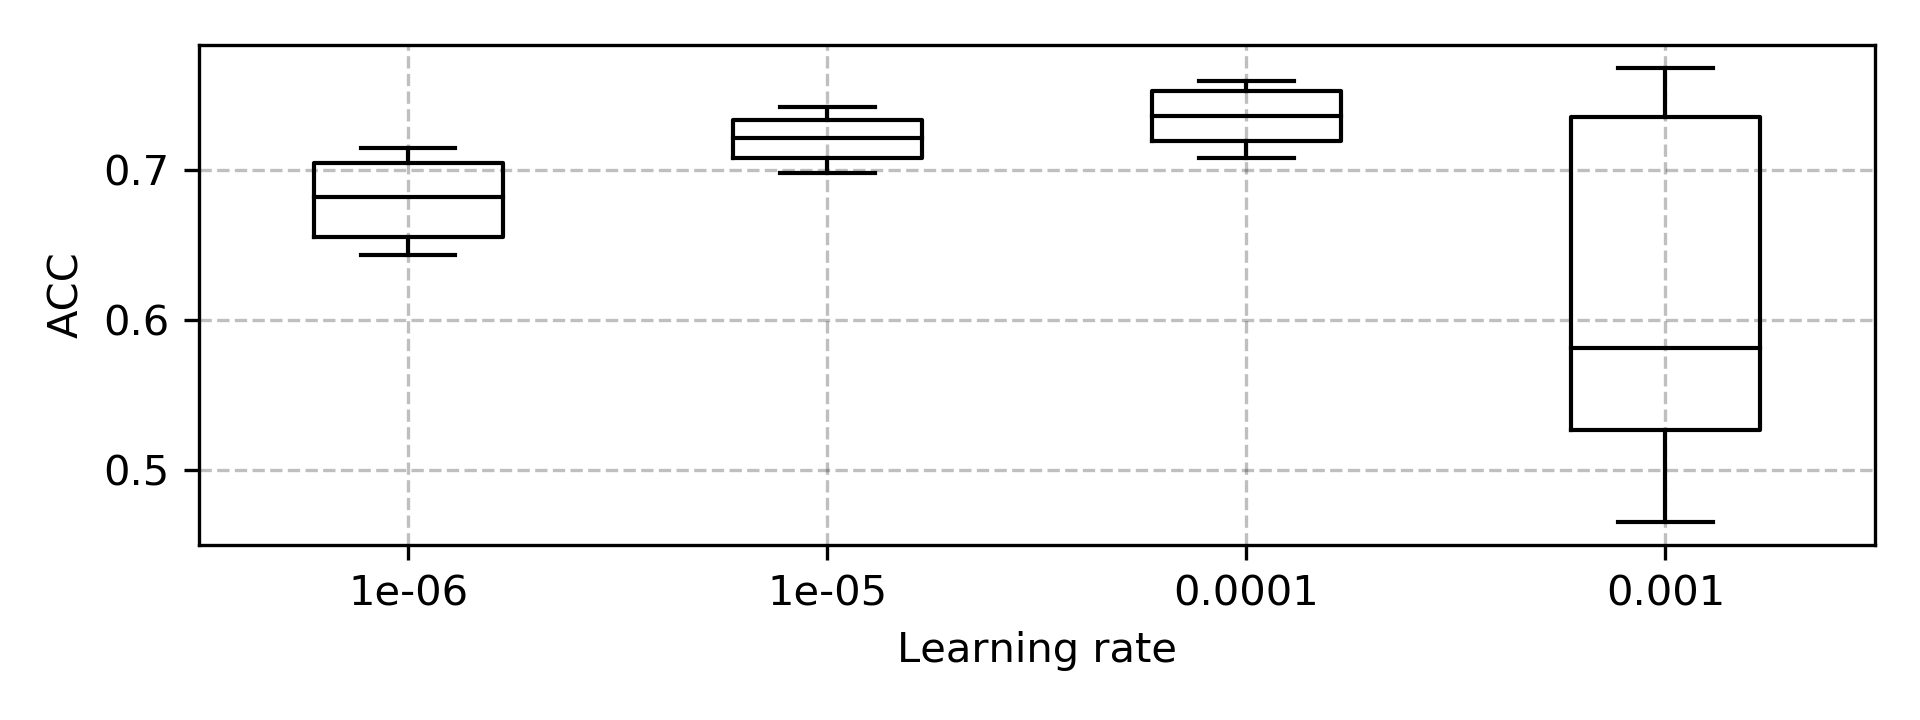
\includegraphics[width=0.7\textwidth]{mtask/densenet121_ulb_anapath_lba_learning_rate_main.png}
    \caption{Distributions of scores per learning rate on DenseNet121 with HumanLba dataset. Each boxplot results from the aggregation of the transfer scores of all models using the same learning rate value on the given network and dataset.}
    \label{fig:mtask:lr_effect}
\end{figure}

\begin{figure}[t]
    \centering
    \begin{subfigure}[t]{0.70\textwidth}
        \centering
        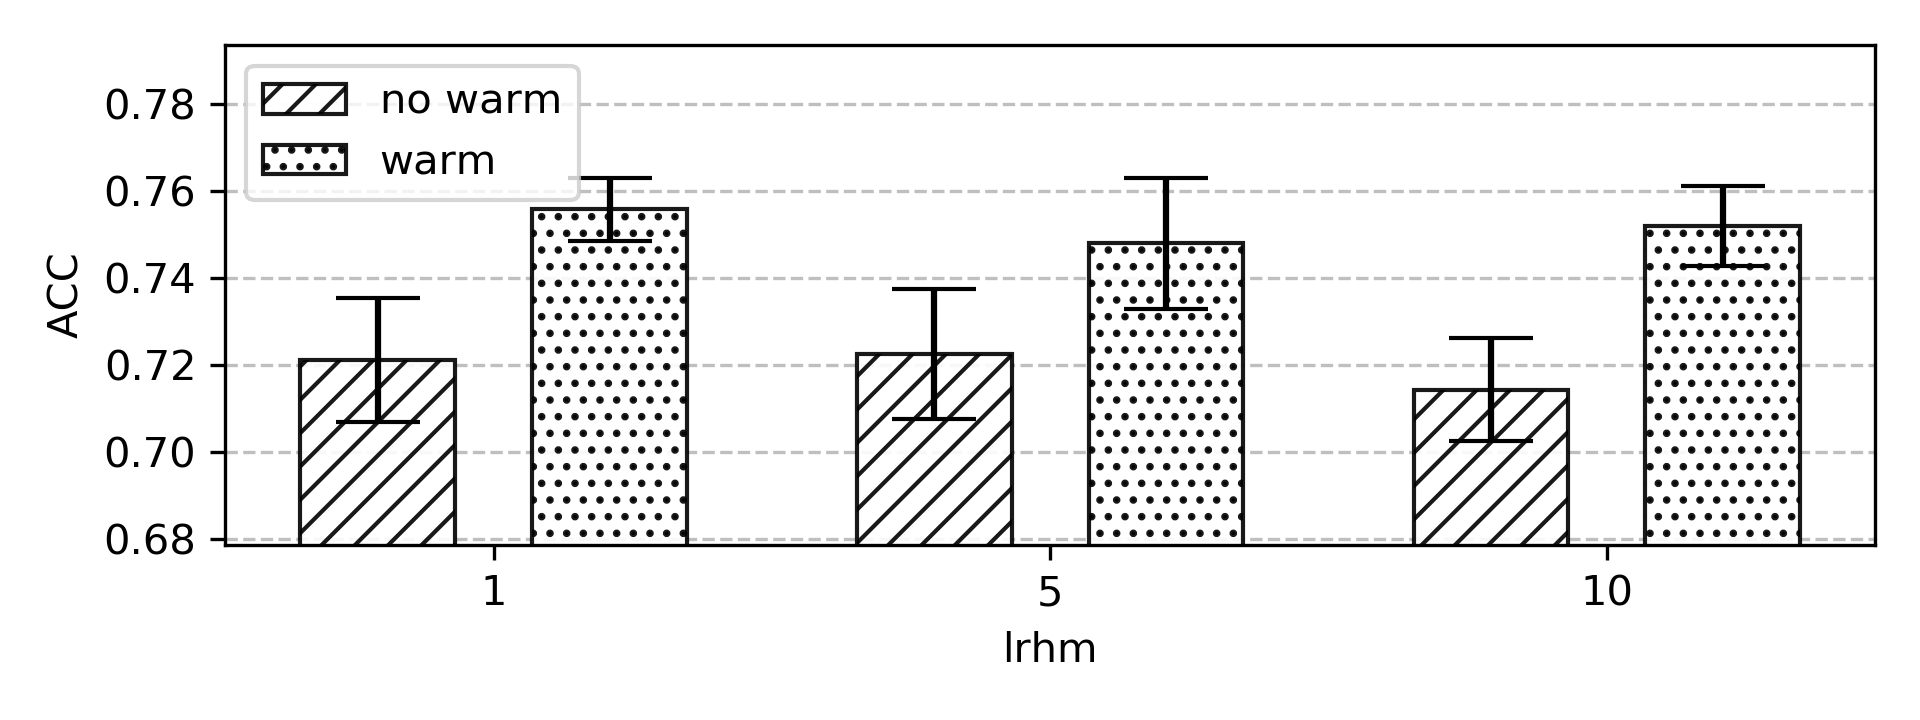
\includegraphics[width=\textwidth]{mtask/bar_lrhm_1e-4_densenet121_ulb_anapath_lba.png}
        \caption{HumanLba}
    \end{subfigure}    
    \begin{subfigure}[t]{0.70\textwidth}
        \centering
        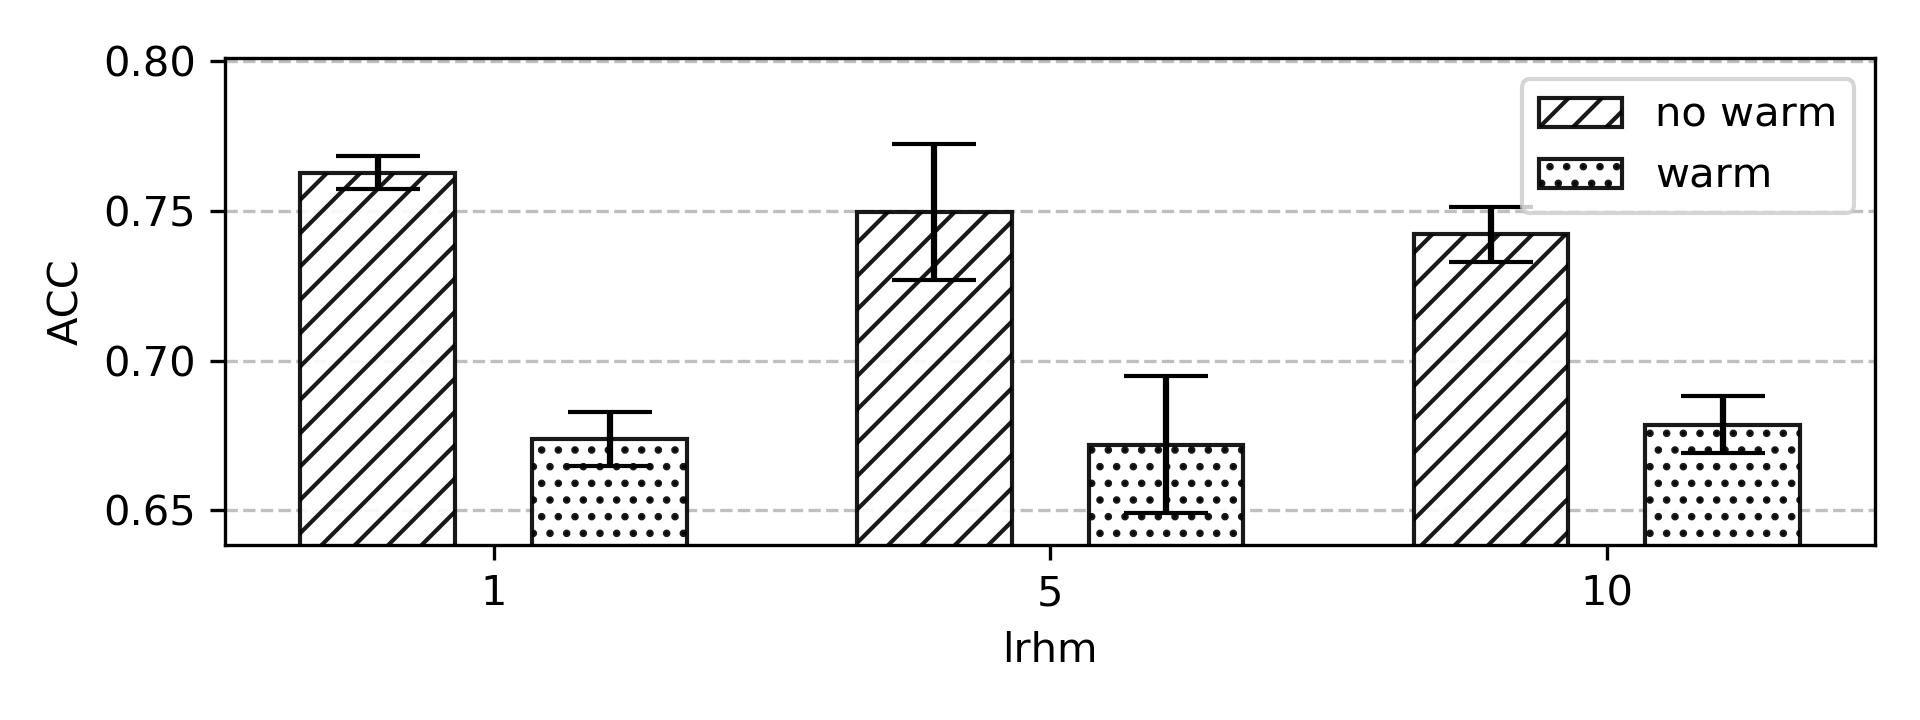
\includegraphics[width=\textwidth]{mtask/bar_lrhm_1e-4_densenet121_ulg_lbtd_lba.png}
        \caption{MouseLba}
    \end{subfigure}    
    \caption{Transfer performance for combinations of the hyperparameters $\gamma_\tau$ (learning rate heads multiplier, \textit{lrhm}) and $w$ (warm up) on two different datasets with learning rate $\gamma = 10^{-4}$ on DenseNet121. Error bars report twice the standard deviation.}
    \label{fig:mtask:hyper_other_effect}
\end{figure}

Our experiments have shown that the hyperparameter impacting transfer performance the most was the multi-task training learning rate. Figure \ref{fig:mtask:lr_effect} shows the distributions of scores per learning rate using DenseNet121 and \textit{HumanLba} dataset. We have picked this plot specifically because it exhibits the most frequent pattern regarding the effect of the learning rate. Similar plots for other datasets as well as ResNet50 can be found in Supplementary Figure \ref{app:mtask:fig:lr_resnet}. We have observed that the highest learning rate $10^{-3}$ yielded highly variable performance where were most of the time inferior compared to lower learning rates. It indicates that this specific value is too high to cope with the multi-task setting as it prevents the models from making use of the tasks information efficiently. This is likely due to training instabilities (convergence issues, noisy training loss) and overfitting. It appears that the lowest learning rate $10^{-6}$, although yielding more stable performance, generally underperforms higher learning rates $10^{-5}$ and $10^{-4}$. For both networks and most datasets, the latter learning rate $10^{-4}$ is the best performing on average.

The impact of the two other hyperparameters $\tau_\gamma$ and $w$ seems to be minor for most datasets as variation stays within two standard deviations. Moreover, there is no pattern emerging from our experiments regarding those hyperparameters in general. Two exceptions to this observation are the \textit{HumanLba} and \textit{MouseLba} datasets which exhibit significant performance variations on both networks. The variations are shown in Figure \ref{fig:mtask:hyper_other_effect} (similar figures can be found for other networks and datasets in Supplementary Figures \ref{app:mtask:fig:bar_lrhm_densenet} and \ref{app:mtask:fig:bar_lrhm_resnet}). Those Figures show that \textit{HumanLba} benefits from warming up whereas \textit{MouseLba} performance are hurt. This indicates that the effect on transfer performance of warming up and multiplying heads learning rate is very dataset dependent and no general rule can be drawn from our experiments.

\subsection{Evaluation of released multi-task pre-trained models}
\label{ssec:mtask:breakhis_eval}

\begin{table}
    \centering
    \small
    \begin{tabular}{|c|c|c|cccc|}
        \hline
        Tr. & Network & Source & 40x & 100x & 200x & 400x \\
        \hline
\multirow{6}{*}{FE} & \multirow{2}{*}{DenseNet121} & ImageNet & $85.83 \pm 2.58$ & $85.38 \pm 4.14$ & $84.50 \pm 1.73$ & $84.81 \pm 1.26$\\
& & Multi-task & $86.05 \pm 2.51$ & $84.74 \pm 3.83$ & $85.75 \pm 2.64$ & $87.22 \pm 1.65$\\
\cline{2-7}
& \multirow{2}{*}{ResNet50} & ImageNet & $85.42 \pm 3.56$ & $84.20 \pm 3.18$ & $86.40 \pm 3.45$ & $82.64 \pm 1.16$\\
& & Multi-task & $84.77 \pm 3.76$ & $83.95 \pm 2.25$ & $89.15 \pm 4.40$ & $86.86 \pm 2.76$\\
\cline{2-7}
&  \multicolumn{2}{c|}{(1) (Decaf)} &  $84.00 \pm 6.90 $ & $83.90  \pm 5.90$ & $86.30 \pm 3.50$ & $82.10 \pm 2.40$ \\
& \multicolumn{2}{c|}{(2) (VGG-VD)} & $86.90 \pm 5.20$ & $85.40 \pm 5.70$ & $85.20 \pm 4.40$ & $85.70 \pm 8.80$ \\
\hline
\multirow{4}{*}{FT} & \multirow{2}{*}{DenseNet121} & ImageNet & $83.64 \pm 5.78$ & $85.99 \pm 4.22$ & $89.07 \pm 3.45$ & $85.38 \pm 3.89$\\
& & Multi-task & $82.69 \pm 6.22$ & $86.32 \pm 1.08$ & $90.91 \pm 3.07$ & $85.74 \pm 3.44$\\
\cline{2-7}
& \multirow{2}{*}{ResNet50} & ImageNet & $84.43 \pm 5.48$ & $83.13 \pm 2.76$ & $88.96 \pm 3.27$ & $84.08 \pm 2.39$\\
& & Multi-task & $85.83 \pm 4.05$ & $84.51 \pm 3.46$ & $87.99 \pm 3.34$ & $84.10 \pm 4.00$\\
%\multicolumn{2}{|c}{\citeauthor{song2017supervised} \cite{song2017supervised}} & VGG-VD+ & $90.20 \pm 3.20$ & $91.20 \pm 4.40$ & $87.80 \pm 5.30$ & $87.40 \pm 7.20$ \\
        \hline
    \end{tabular}
    \caption{Transfer performance of our best multi-task pre-trained model on the BreakHis datasets using \textbf{feature extraction} (FE) and \textbf{fine-tuning} (FT). Average per-patient accuracies and standard deviations are given per magnification (x40, x100, x200 and x400). \textbf{(1)} \cite{spanhol2017deep}, \textbf{(2)} \cite{song2017supervised}.}
    \label{tab:mtask:breakhis_eval}
\end{table}

With the idea of releasing the best multi-task pre-trained models to the community, we have re-trained each network one time using the same procedure described in the paper and the best hyperparameters found using the ranks. Especially, for DenseNet121, we have picked $\gamma = 10^{-4}$, $\tau_\gamma = 5$ and warm up. For ResNet50, we have picked $\gamma = 10^{-3}$, $\tau_\gamma = 1$ and warm up. We have used all the data available for re-training (\ie the training, validation and test sets of our 22 tasks).

In order to evaluate the to-be released models, we kept the BreakHis dataset \cite{spanhol2015dataset} out of our pool. We have transferred the two resulting models using both feature extraction and fine-tuning as presented in the article. The transfer was repeated on the five original per-patient folds of BreakHis and performance was averaged over those folds. The resulting transfer scores are given in Table \ref{tab:mtask:breakhis_eval}. We have not compared our approach to the full BreakHis benchmark but only to similar methods of transfer learning of which we have found two \cite{spanhol2017deep, song2017supervised} that perform feature extraction.

Our conclusions do not change. For feature extraction, our approach either improves over ImageNet transfer or provides similar performance. We have observed that our method yield better performance on higher magnification in particular. Our transfer learning approach is also on par with similar ones from the literature.

For fine-tuning, there does not seem to be a significant difference between our approach and ImageNet. Surprisingly, we have also observed that fine-tuning (from ImageNet or our models) yielded inferior performance compared to feature extraction in some cases which could be explained by the fact that our protocol requires a validation set for tuning the fine-tuning hyperparameters. To avoid reducing too much the size of the training set, we have extracted a small validation set (approximately $10\%$ of the whole data) which might be too small for robust selection, especially when coupled with a reduced training set.

\subsection{Discussion and future works}
\label{ssec:mtask:res:discussion}

Features extracted from our models are in general superior to ImageNet ones %(see feature extraction results in Section \ref{ssec:mtask:transfer_perfromance})
which shows that multi-task pre-training is effective at creating task-specific features. This important observation confirms the conclusions of previous works that domain-specific pre-training is a good idea and also validates the multi-task approach when a large source dataset is not available. 

The second important observation is that fine-tuning does not benefit from using our models as we obtain similar transfer performance whatever the source. This indicates that fine-tuning is able to recover the lack of specificity of ImageNet features compared to ours. It contradicts our initial hypothesis that transfer should work better when source and target domains are similar. There might be several reasons why we observe such phenomenon. First, \citeauthor{yosinski2014transferable} \cite{yosinski2014transferable}, who concluded about the importance of task similarity for efficient transfer, performed their experiments on simple architectures (\eg simple stack of convolutional layers). In our case, we have used more recent architectures (\ie residual and densely connected networks) which are easier to train and might be less impacted by their initial weights. Second, most previous works have shown that fine-tuning was beneficial in a single source task transfer scenario exclusively. Our multi-task pre-training is able to learn specific features but we cannot exclude that a more advanced approach could result in even stronger features. This might change our conclusion that fine-tuning does not benefit from \acrshort{mtl} transfer. For instance, some papers have highlighted training difficulties associated with multi-task (\eg gradients interference \cite{yu2020gradient}) and \acrlong{tl} (\eg batch normalization \cite{chang2019domain}) that could be investigated in our context. In addition, it is likely that, given a target task, not all tasks in the pool contribute equally to transfer performance. A negative transfer phenomenon might even be at play and some tasks might have a destructive effect during the pre-training phase (\ie if they were removed, transfer performance would increase). Incorporating a training mechanism that could dynamically increase (\textit{resp.} decrease) the contribution of constructive (\textit{resp.} destructive) tasks would certainly help improving the resulting features. Alternatively, instead of using all the tasks, one could find a mechanism for selecting a subset of (the most relevant) source tasks for a given target task. Such solution would entail however a significant additional computational cost, since a new \acrshort{mtl} model would have to be trained for each new target task.

There are also several interesting research directions regarding the architecture. On the one hand, it would be interesting to study the effect of increasing the capacity of the task-specific parts. On the other hand, we have only worked with classification tasks so far but it is possible to incorporate directly segmentation or detection tasks to the pre-training by appending an ad-hoc network as a head. Hopefully, enriching the training signal with a dense prediction task such as segmentation could improve the transferability of the resulting models. However, this approach also raises pratical questions and issues such as model memory usage or loss aggregation. 

\section{Conclusion}

We have investigated the use of multi-task learning for pre-training neural networks in \acrlong{dp}. We have first created a pool of classification tasks from existing sources containing almost 900k \acrlong{dp} images. Using this pool, we have pre-trained a neural network in a multi-task setting in order to transfer the resulting model to unseen \acrlong{dp} tasks. Using a robust evaluation protocol, we have shown that transferring a model pre-trained in multi-task can be beneficial for the performance on the target task. When compared to transfer from ImageNet, our pre-training approach coupled with feature extraction yields comparable or better performance depending on the target dataset. We have observed that fine-tuning multi-task or ImageNet pre-trained models yields comparable performance. It suggests that fine-tuning is able to recover from the lack of feature specificity whatever the pre-training source. However, pre-training remains crucial, as models trained from scratch are clearly inferior. 
